\chapter{Supporting Materials}
\begin{table}[]
	\caption{List of hyperparameters used for experiments }
	\label{tab:hyperparams}
	\center
	\begin{tabular}{|c|c|}
		\hline
		\multicolumn{2}{|c|}{\textbf{Optimization Parameters}} \\ \hline
		Optimizer                        & Adam                \\ \hline
		Learning Rate                    & 0.0003              \\ \hline
		KL Annealing Schedule            & 80,000 steps        \\ \hline
		Word Dropout Rate                & 0.1                 \\ \hline
		Clip nNorm                        & 1.0                 \\ \hline
		Mini Batch Size                  & 64                  \\ \hline
		Number of Samples (ELBO)         & 10                  \\ \hline
		\multicolumn{2}{|c|}{\textbf{Model Parameters}}                 \\ \hline
		Source Embedding Size            & 256                 \\ \hline
		Target Embedding Size            & 256                 \\ \hline
		Encoder Hidden Dimensions        & 256                 \\ \hline
		Number of Encoder Layers         & 1                   \\ \hline
		Decoder Hidden Dimensions        & 256                 \\ \hline
		Number of Decoder Layers         & 1                   \\ \hline
		Dropout                          & 0.5                 \\ \hline
		Z dim (latent variable)          & 2, 128, 256        \\ \hline
		\multicolumn{2}{|c|}{\textbf{Global Attention Mechanism}}       \\ \hline
		Key Size                         & 512                 \\ \hline
		Query Size                       & 256                 \\ \hline
		\multicolumn{2}{|c|}{\textbf{IAF Details}}                    \\ \hline
		Autoregressive NN hidden sizes                & 320, 320 \\ \hline
		\multicolumn{2}{|c|}{\textbf{Planar Flows Details}}             \\ \hline
		Hidden layer dimensions          & 150                 \\ \hline
	\end{tabular}
\end{table}



\begin{table}[]
	\caption{IWSLT sentence counts for De--En language pair. Counts represent actual number of sentences we use in our analysis when limiting max sentence length to 50. Values in parentheses represent full sentence counts of each dataset.} 
	\center
	\begin{tabular}{|l|l|}
		\hline
		\multicolumn{2}{|c|}{De--EN} \\ \hline
		Train    & 182999 (233213)   \\ \hline
		Dev      & 1873 (2052)       \\ \hline
		Test     & 9101  (9773)      \\ \hline
	\end{tabular}
\end{table}

\section{Discussion on other latent dimensions}

In this section we include our results when the latent space was set to 2. These results are available in Table \ref{tab:de_en_besttranslations_supp}. We originally considered such a small latent space for plotting purposes, but found it to be quite effective. Our findings would seem congruent with previous results on the value of smaller latent spaces \cite{schulz2018StochasticDecoder}.\footnote{We do not know if other researchers have also considered such small latent spaces. } Interestingly, our conclusions with flow complexity are reverse for this latent space where mostly planar flows perform better than \ac{IAF}. This would suggest for especially small latent spaces, that flexible transformations are more of a hindrance than beneficial to translation performance. We chose to exclude this result from the main thesis because to our knowledge there is no precedence for such performance gains, and further future work is necessary.

We also considered the same drop in performance scenario discussed in the main thesis. The KL divergence results are in Table~\ref{tab:de_en_kl_divergence_sup}. The BLEU difference are in Table~\ref{tab:de_en_delta_bleu_sup}. Here, we see similar trends as in the original models where performance drops are quite small with the latent variable $z$. For most \ac{VNMT} models we again see that the latent variable seems to negatively impact performance with $z=2$. 
 
Additionally, we visualized the latent space of several sentence pairs as the latent dimensions were quite small. Our \ac{VNMT} results are available in Figures~\ref{fig:vnmt_planar} and ~\ref{fig:vnmt_iaf}. Our \ac{GNMT} results are available in Figures~\ref{fig:gnmt_planar} and ~\ref{fig:gnmt_iaf}. These plots were generated by first encoding each sentence pair to produce the variational posterior parameters. With these parameters, we generated 10,000 samples from the distributions. Each plot is then a Gaussian kernel density estimation of the samples after being transformed by K normalizing flows with the base distribution on the far left, and $k=8$ flows on the far right. These plots largely show us the expected behaviours of the transformations. In the planar flows cases we see mostly the distribution being shifted around in the latent space but otherwise remaining uni-modal. In the \ac{IAF} cases we see interestingly that the normalizing flows are collapsing our 2D latent spaces into 1D. This may be an indication that the stochastic nature of the latent variable is actually negatively impacting the training as the \ac{IAF} flows attempt to flatten the distribution. 



\begin{table}[] 
	\caption{BLEU score for our models with normalizing flows for De-En translation. The best performing models are in bold for each type and number of flows. This table is similar to Table~\ref{tab:de_en_besttranslations} in main thesis, but includes result for latent dimensions set to 2. }
	\label{tab:de_en_besttranslations_supp}
	\center
	\begin{tabular}{llllllcl}
		\multicolumn{8}{c}{\textbf{Latent Dimension: 2}}                                                                                                                                                                                                                                                                                                                                                                                                                                                                                                   \\ \hline
		\multicolumn{1}{|l|}{\textbf{Flows}}                          & \multicolumn{1}{l|}{\textbf{1}}                             & \multicolumn{1}{l|}{\textbf{2}}                             & \multicolumn{1}{l|}{\textbf{4}}                             & \multicolumn{1}{l|}{\textbf{8}}                             & \multicolumn{1}{l|}{\textbf{16}}                            & \multicolumn{1}{l|}{\textbf{0 (Baseline)}}                                    & \multicolumn{1}{c|}{\textbf{Model}}                                          \\ \hline
		\rowcolor[HTML]{F9F9E1} 
		\multicolumn{1}{|l|}{\cellcolor[HTML]{F9F9E1}Planar}          & \multicolumn{1}{l|}{\cellcolor[HTML]{F9F9E1}\textbf{19.06}} & \multicolumn{1}{l|}{\cellcolor[HTML]{F9F9E1}18.95}          & \multicolumn{1}{l|}{\cellcolor[HTML]{F9F9E1}18.94}          & \multicolumn{1}{l|}{\cellcolor[HTML]{F9F9E1}19.01}          & \multicolumn{1}{l|}{\cellcolor[HTML]{F9F9E1}19.05}          & \multicolumn{1}{c|}{\cellcolor[HTML]{F9F9E1}}                                 & \multicolumn{1}{l|}{\cellcolor[HTML]{F9F9E1}}                                \\ \cline{1-6}
		\rowcolor[HTML]{F9F9E1} 
		\multicolumn{1}{|l|}{\cellcolor[HTML]{F9F9E1}IAF}             & \multicolumn{1}{l|}{\cellcolor[HTML]{F9F9E1}18.89}          & \multicolumn{1}{l|}{\cellcolor[HTML]{F9F9E1}18.48}          & \multicolumn{1}{l|}{\cellcolor[HTML]{F9F9E1}18.803}         & \multicolumn{1}{l|}{\cellcolor[HTML]{F9F9E1}\textbf{18.96}} & \multicolumn{1}{l|}{\cellcolor[HTML]{F9F9E1}18.67}          & \multicolumn{1}{c|}{\multirow{-2}{*}{\cellcolor[HTML]{F9F9E1}18.92}}          & \multicolumn{1}{l|}{\multirow{-2}{*}{\cellcolor[HTML]{F9F9E1}VNMT}}          \\ \hline
		\rowcolor[HTML]{F4DAD8} 
		\multicolumn{1}{|l|}{\cellcolor[HTML]{F4DAD8}Planar}          & \multicolumn{1}{l|}{\cellcolor[HTML]{F4DAD8}20.77}          & \multicolumn{1}{l|}{\cellcolor[HTML]{F4DAD8}20.70}          & \multicolumn{1}{l|}{\cellcolor[HTML]{F4DAD8}20.81}          & \multicolumn{1}{l|}{\cellcolor[HTML]{F4DAD8}20.86}          & \multicolumn{1}{l|}{\cellcolor[HTML]{F4DAD8}20.37}          & \multicolumn{1}{c|}{\cellcolor[HTML]{F4DAD8}}                                 & \multicolumn{1}{l|}{\cellcolor[HTML]{F4DAD8}}                                \\ \cline{1-6}
		\rowcolor[HTML]{F4DAD8} 
		\multicolumn{1}{|l|}{\cellcolor[HTML]{F4DAD8}IAF}             & \multicolumn{1}{l|}{\cellcolor[HTML]{F4DAD8}20.61}          & \multicolumn{1}{l|}{\cellcolor[HTML]{F4DAD8}20.52}          & \multicolumn{1}{l|}{\cellcolor[HTML]{F4DAD8}20.58}          & \multicolumn{1}{l|}{\cellcolor[HTML]{F4DAD8}20.55}          & \multicolumn{1}{l|}{\cellcolor[HTML]{F4DAD8}20.46}          & \multicolumn{1}{c|}{\multirow{-2}{*}{\cellcolor[HTML]{F4DAD8}\textbf{21.02}}} & \multicolumn{1}{l|}{\multirow{-2}{*}{\cellcolor[HTML]{F4DAD8}GNMT}}          \\ \hline
		\multicolumn{8}{c}{\textbf{Latent Dimension: 128}}                                                                                                                                                                                                                                                                                                                                                                                                                                                                                                 \\ \hline
		\multicolumn{1}{|l|}{\textbf{Flows}}                          & \multicolumn{1}{l|}{\textbf{1}}                             & \multicolumn{1}{l|}{\textbf{2}}                             & \multicolumn{1}{l|}{\textbf{4}}                             & \multicolumn{1}{l|}{\textbf{8}}                             & \multicolumn{1}{l|}{\textbf{16}}                            & \multicolumn{1}{l|}{\textbf{0 (Baseline)}}                                    & \multicolumn{1}{l|}{\textbf{Model}}                                          \\ \hline
		\rowcolor[HTML]{F9F9E1} 
		\multicolumn{1}{|l|}{\cellcolor[HTML]{F9F9E1}Planar}          & \multicolumn{1}{l|}{\cellcolor[HTML]{F9F9E1}18.84}          & \multicolumn{1}{l|}{\cellcolor[HTML]{F9F9E1}18.84}          & \multicolumn{1}{l|}{\cellcolor[HTML]{F9F9E1}19.14}          & \multicolumn{1}{l|}{\cellcolor[HTML]{F9F9E1}19.02}          & \multicolumn{1}{l|}{\cellcolor[HTML]{F9F9E1}\textbf{19.18}} & \multicolumn{1}{c|}{\cellcolor[HTML]{F9F9E1}}                                 & \multicolumn{1}{l|}{\cellcolor[HTML]{F9F9E1}}                                \\ \cline{1-6}
		\rowcolor[HTML]{F9F9E1} 
		\multicolumn{1}{|l|}{\cellcolor[HTML]{F9F9E1}IAF}             & \multicolumn{1}{l|}{\cellcolor[HTML]{F9F9E1}18.89}          & \multicolumn{1}{l|}{\cellcolor[HTML]{F9F9E1}18.96}          & \multicolumn{1}{l|}{\cellcolor[HTML]{F9F9E1}\textbf{19.29}} & \multicolumn{1}{l|}{\cellcolor[HTML]{F9F9E1}18.81}          & \multicolumn{1}{l|}{\cellcolor[HTML]{F9F9E1}18.92}          & \multicolumn{1}{c|}{\multirow{-2}{*}{\cellcolor[HTML]{F9F9E1}18.768}}         & \multicolumn{1}{l|}{\multirow{-2}{*}{\cellcolor[HTML]{F9F9E1}VNMT}}          \\ \hline
		\rowcolor[HTML]{F4DAD8} 
		\multicolumn{1}{|l|}{\cellcolor[HTML]{F4DAD8}Planar}          & \multicolumn{1}{l|}{\cellcolor[HTML]{F4DAD8}20.59}          & \multicolumn{1}{l|}{\cellcolor[HTML]{F4DAD8}20.60}          & \multicolumn{1}{l|}{\cellcolor[HTML]{F4DAD8}20.48}          & \multicolumn{1}{l|}{\cellcolor[HTML]{F4DAD8}20.55}          & \multicolumn{1}{l|}{\cellcolor[HTML]{F4DAD8}20.66}          & \multicolumn{1}{c|}{\cellcolor[HTML]{F4DAD8}}                                 & \multicolumn{1}{l|}{\cellcolor[HTML]{F4DAD8}}                                \\ \cline{1-6}
		\rowcolor[HTML]{F4DAD8} 
		\multicolumn{1}{|l|}{\cellcolor[HTML]{F4DAD8}IAF}             & \multicolumn{1}{l|}{\cellcolor[HTML]{F4DAD8}20.64}          & \multicolumn{1}{l|}{\cellcolor[HTML]{F4DAD8}20.64}          & \multicolumn{1}{l|}{\cellcolor[HTML]{F4DAD8}20.51}          & \multicolumn{1}{l|}{\cellcolor[HTML]{F4DAD8}20.65}          & \multicolumn{1}{l|}{\cellcolor[HTML]{F4DAD8}20.50}          & \multicolumn{1}{c|}{\multirow{-2}{*}{\cellcolor[HTML]{F4DAD8}\textbf{20.73}}} & \multicolumn{1}{l|}{\multirow{-2}{*}{\cellcolor[HTML]{F4DAD8}GNMT}}          \\ \hline
		\multicolumn{8}{c}{\textbf{Latent Dimension: 256}}                                                                                                                                                                                                                                                                                                                                                                                                                                                                                                 \\ \hline
		\multicolumn{1}{|l|}{\textbf{Flows}}                          & \multicolumn{1}{l|}{\textbf{1}}                             & \multicolumn{1}{l|}{\textbf{2}}                             & \multicolumn{1}{l|}{\textbf{4}}                             & \multicolumn{1}{l|}{\textbf{8}}                             & \multicolumn{1}{l|}{\textbf{16}}                            & \multicolumn{1}{l|}{\textbf{0 (Baseline)}}                                    & \multicolumn{1}{l|}{\textbf{Model}}                                          \\ \hline
		\rowcolor[HTML]{F9F9E1} 
		\multicolumn{1}{|l|}{\cellcolor[HTML]{F9F9E1}Planar} & \multicolumn{1}{l|}{\cellcolor[HTML]{F9F9E1}18.93}          & \multicolumn{1}{l|}{\cellcolor[HTML]{F9F9E1}\textbf{19.26}} & \multicolumn{1}{l|}{\cellcolor[HTML]{F9F9E1}19.02}          & \multicolumn{1}{l|}{\cellcolor[HTML]{F9F9E1}18.80}          & \multicolumn{1}{l|}{\cellcolor[HTML]{F9F9E1}18.82}          & \multicolumn{1}{c|}{\cellcolor[HTML]{F9F9E1}}                                 & \multicolumn{1}{l|}{\cellcolor[HTML]{F9F9E1}}                                \\ \cline{1-6}
		\rowcolor[HTML]{F9F9E1} 
		\multicolumn{1}{|l|}{\cellcolor[HTML]{F9F9E1}IAF}    & \multicolumn{1}{l|}{\cellcolor[HTML]{F9F9E1}18.95}          & \multicolumn{1}{l|}{\cellcolor[HTML]{F9F9E1}\textbf{19.17}} & \multicolumn{1}{l|}{\cellcolor[HTML]{F9F9E1}19.02}          & \multicolumn{1}{l|}{\cellcolor[HTML]{F9F9E1}18.99}          & \multicolumn{1}{l|}{\cellcolor[HTML]{F9F9E1}18.77}          & \multicolumn{1}{c|}{\multirow{-2}{*}{\cellcolor[HTML]{F9F9E1}18.76}}          & \multicolumn{1}{l|}{\multirow{-2}{*}{\cellcolor[HTML]{F9F9E1} VNMT}} \\ \hline
		\rowcolor[HTML]{F4DAD8} 
		\multicolumn{1}{|l|}{\cellcolor[HTML]{F4DAD8}Planar} & \multicolumn{1}{l|}{\cellcolor[HTML]{F4DAD8}20.55}          & \multicolumn{1}{l|}{\cellcolor[HTML]{F4DAD8}\textbf{20.67}} & \multicolumn{1}{l|}{\cellcolor[HTML]{F4DAD8}20.54}          & \multicolumn{1}{l|}{\cellcolor[HTML]{F4DAD8}20.51}          & \multicolumn{1}{l|}{\cellcolor[HTML]{F4DAD8}\textbf{20.67}} & \multicolumn{1}{c|}{\cellcolor[HTML]{F4DAD8}}                                 & \multicolumn{1}{l|}{\cellcolor[HTML]{F4DAD8}}                                \\ \cline{1-6}
		\rowcolor[HTML]{F4DAD8} 
		\multicolumn{1}{|l|}{\cellcolor[HTML]{F4DAD8}IAF}    & \multicolumn{1}{l|}{\cellcolor[HTML]{F4DAD8}20.85}          & \multicolumn{1}{l|}{\cellcolor[HTML]{F4DAD8}\textbf{20.86}} & \multicolumn{1}{l|}{\cellcolor[HTML]{F4DAD8}20.64}          & \multicolumn{1}{l|}{\cellcolor[HTML]{F4DAD8}20.62}          & \multicolumn{1}{l|}{\cellcolor[HTML]{F4DAD8}20.66}          & \multicolumn{1}{c|}{\multirow{-2}{*}{\cellcolor[HTML]{F4DAD8}20.66}}          & \multicolumn{1}{l|}{\multirow{-2}{*}{\cellcolor[HTML]{F4DAD8}GNMT}} \\ \hline
	\end{tabular}
\end{table}



\begin{table}
	\caption{Average KL divergence for the test set. For \ac{VNMT} the KL term should be smaller meaning the distributions encode similar information. For \ac{GNMT} they should be higher as these suggest more informative latent spaces.  }
	\label{tab:de_en_kl_divergence_sup}
	\center
	\begin{tabular}{lccccccl}
		\multicolumn{8}{c}{\textbf{Latent Dimension: 2 (KL Difference)}}                                                                                                                                                                                                                                                                                                                                                                                                                      \\ \hline
		\multicolumn{1}{|l|}{\textbf{Flows}}                       & \multicolumn{1}{c|}{\textbf{1}}                   & \multicolumn{1}{c|}{\textbf{2}}                   & \multicolumn{1}{c|}{\textbf{4}}                    & \multicolumn{1}{c|}{\textbf{8}}                   & \multicolumn{1}{c|}{\textbf{16}}                   & \multicolumn{1}{c|}{\textbf{0 (Baseline)}}                          & \multicolumn{1}{c|}{\textbf{Model}}                                          \\ \hline
		\rowcolor[HTML]{F9F9E1} 
		\multicolumn{1}{|l|}{\cellcolor[HTML]{F9F9E1}Planar}       & \multicolumn{1}{c|}{\cellcolor[HTML]{F9F9E1}0.94} & \multicolumn{1}{c|}{\cellcolor[HTML]{F9F9E1}1.45} & \multicolumn{1}{c|}{\cellcolor[HTML]{F9F9E1}0.68}  & \multicolumn{1}{c|}{\cellcolor[HTML]{F9F9E1}0.0}  & \multicolumn{1}{c|}{\cellcolor[HTML]{F9F9E1}0.0}   & \multicolumn{1}{c|}{\cellcolor[HTML]{F9F9E1}}                       & \multicolumn{1}{l|}{\cellcolor[HTML]{F9F9E1}}                                \\ \cline{1-6}
		\rowcolor[HTML]{F9F9E1} 
		\multicolumn{1}{|l|}{\cellcolor[HTML]{F9F9E1}IAF}          & \multicolumn{1}{c|}{\cellcolor[HTML]{F9F9E1}1.15} & \multicolumn{1}{c|}{\cellcolor[HTML]{F9F9E1}1.56} & \multicolumn{1}{c|}{\cellcolor[HTML]{F9F9E1}1.4}   & \multicolumn{1}{c|}{\cellcolor[HTML]{F9F9E1}0.85} & \multicolumn{1}{c|}{\cellcolor[HTML]{F9F9E1}1.56}  & \multicolumn{1}{c|}{\multirow{-2}{*}{\cellcolor[HTML]{F9F9E1}1.15}} & \multicolumn{1}{l|}{\multirow{-2}{*}{\cellcolor[HTML]{F9F9E1}VNMT}}          \\ \hline
		\rowcolor[HTML]{F4DAD8} 
		\multicolumn{1}{|l|}{\cellcolor[HTML]{F4DAD8}Planar}       & \multicolumn{1}{c|}{\cellcolor[HTML]{F4DAD8}2.48} & \multicolumn{1}{c|}{\cellcolor[HTML]{F4DAD8}2.32} & \multicolumn{1}{c|}{\cellcolor[HTML]{F4DAD8}2.01}  & \multicolumn{1}{c|}{\cellcolor[HTML]{F4DAD8}0.10} & \multicolumn{1}{c|}{\cellcolor[HTML]{F4DAD8}3.64}  & \multicolumn{1}{c|}{\cellcolor[HTML]{F4DAD8}}                       & \multicolumn{1}{l|}{\cellcolor[HTML]{F4DAD8}}                                \\ \cline{1-6}
		\rowcolor[HTML]{F4DAD8} 
		\multicolumn{1}{|l|}{\cellcolor[HTML]{F4DAD8}IAF}          & \multicolumn{1}{c|}{\cellcolor[HTML]{F4DAD8}0.0}  & \multicolumn{1}{c|}{\cellcolor[HTML]{F4DAD8}2.36} & \multicolumn{1}{c|}{\cellcolor[HTML]{F4DAD8}3.91}  & \multicolumn{1}{c|}{\cellcolor[HTML]{F4DAD8}2.09} & \multicolumn{1}{c|}{\cellcolor[HTML]{F4DAD8}2.63}  & \multicolumn{1}{c|}{\multirow{-2}{*}{\cellcolor[HTML]{F4DAD8}2.99}} & \multicolumn{1}{l|}{\multirow{-2}{*}{\cellcolor[HTML]{F4DAD8}GNMT}}          \\ \hline
		\multicolumn{8}{c}{\textbf{Latent Dimension: 128 (KL Difference)}}                                                                                                                                                                                                                                                                                                                                                                                                                    \\ \hline
		\multicolumn{1}{|l|}{\textbf{Flows}}                       & \multicolumn{1}{c|}{\textbf{1}}                   & \multicolumn{1}{c|}{\textbf{2}}                   & \multicolumn{1}{c|}{\textbf{4}}                    & \multicolumn{1}{c|}{\textbf{8}}                   & \multicolumn{1}{c|}{\textbf{16}}                   & \multicolumn{1}{c|}{\textbf{0 (Baseline)}}                          & \multicolumn{1}{l|}{\textbf{Model}}                                          \\ \hline
		\rowcolor[HTML]{F9F9E1} 
		\multicolumn{1}{|l|}{\cellcolor[HTML]{F9F9E1}Planar}       & \multicolumn{1}{c|}{\cellcolor[HTML]{F9F9E1}2.16} & \multicolumn{1}{c|}{\cellcolor[HTML]{F9F9E1}1.27} & \multicolumn{1}{c|}{\cellcolor[HTML]{F9F9E1}1.18}  & \multicolumn{1}{c|}{\cellcolor[HTML]{F9F9E1}1.04} & \multicolumn{1}{c|}{\cellcolor[HTML]{F9F9E1}1.63}  & \multicolumn{1}{c|}{\cellcolor[HTML]{F9F9E1}}                       & \multicolumn{1}{l|}{\cellcolor[HTML]{F9F9E1}}                                \\ \cline{1-6}
		\rowcolor[HTML]{F9F9E1} 
		\multicolumn{1}{|l|}{\cellcolor[HTML]{F9F9E1}IAF}          & \multicolumn{1}{c|}{\cellcolor[HTML]{F9F9E1}0.68} & \multicolumn{1}{c|}{\cellcolor[HTML]{F9F9E1}1.35} & \multicolumn{1}{c|}{\cellcolor[HTML]{F9F9E1}1.32}  & \multicolumn{1}{c|}{\cellcolor[HTML]{F9F9E1}1.6}  & \multicolumn{1}{c|}{\cellcolor[HTML]{F9F9E1}1.06}  & \multicolumn{1}{c|}{\multirow{-2}{*}{\cellcolor[HTML]{F9F9E1}1.04}} & \multicolumn{1}{l|}{\multirow{-2}{*}{\cellcolor[HTML]{F9F9E1}VNMT}}          \\ \hline
		\rowcolor[HTML]{F4DAD8} 
		\multicolumn{1}{|l|}{\cellcolor[HTML]{F4DAD8}Planar}       & \multicolumn{1}{c|}{\cellcolor[HTML]{F4DAD8}3.23} & \multicolumn{1}{c|}{\cellcolor[HTML]{F4DAD8}3.15} & \multicolumn{1}{c|}{\cellcolor[HTML]{F4DAD8}2.36}  & \multicolumn{1}{c|}{\cellcolor[HTML]{F4DAD8}2.82} & \multicolumn{1}{c|}{\cellcolor[HTML]{F4DAD8}3.64}  & \multicolumn{1}{c|}{\cellcolor[HTML]{F4DAD8}}                       & \multicolumn{1}{l|}{\cellcolor[HTML]{F4DAD8}}                                \\ \cline{1-6}
		\rowcolor[HTML]{F4DAD8} 
		\multicolumn{1}{|l|}{\cellcolor[HTML]{F4DAD8}IAF}          & \multicolumn{1}{c|}{\cellcolor[HTML]{F4DAD8}4.31} & \multicolumn{1}{c|}{\cellcolor[HTML]{F4DAD8}4.36} & \multicolumn{1}{c|}{\cellcolor[HTML]{F4DAD8}4.19}  & \multicolumn{1}{c|}{\cellcolor[HTML]{F4DAD8}4.43} & \multicolumn{1}{c|}{\cellcolor[HTML]{F4DAD8}4.14}  & \multicolumn{1}{c|}{\multirow{-2}{*}{\cellcolor[HTML]{F4DAD8}4.39}} & \multicolumn{1}{l|}{\multirow{-2}{*}{\cellcolor[HTML]{F4DAD8}GNMT}}          \\ \hline
		\multicolumn{8}{c}{\textbf{Latent Dimension: 256 (KL Difference)}}                                                                                                                                                                                                                                                                                                                                                                                                                    \\ \hline
		\multicolumn{1}{|l|}{\textbf{Flows}}                       & \multicolumn{1}{c|}{\textbf{1}}                   & \multicolumn{1}{c|}{\textbf{2}}                   & \multicolumn{1}{c|}{\textbf{4}}                    & \multicolumn{1}{c|}{\textbf{8}}                   & \multicolumn{1}{c|}{\textbf{16}}                   & \multicolumn{1}{c|}{\textbf{0 (Baseline)}}                          & \multicolumn{1}{l|}{\textbf{Model}}                                          \\ \hline
		\rowcolor[HTML]{F9F9E1} 
		\multicolumn{1}{|l|}{\cellcolor[HTML]{F9F9E1}Planar}       & \multicolumn{1}{c|}{\cellcolor[HTML]{F9F9E1}0.92} & \multicolumn{1}{c|}{\cellcolor[HTML]{F9F9E1}2.35} & \multicolumn{1}{c|}{\cellcolor[HTML]{F9F9E1}2.37}  & \multicolumn{1}{c|}{\cellcolor[HTML]{F9F9E1}1.11} & \multicolumn{1}{c|}{\cellcolor[HTML]{F9F9E1}1.27}  & \multicolumn{1}{c|}{\cellcolor[HTML]{F9F9E1}}                       & \multicolumn{1}{c|}{\cellcolor[HTML]{F9F9E1}}                                \\ \cline{1-6}
		\rowcolor[HTML]{F9F9E1} 
		\multicolumn{1}{|l|}{\cellcolor[HTML]{F9F9E1}IAF} & \multicolumn{1}{c|}{\cellcolor[HTML]{F9F9E1}2.41} & \multicolumn{1}{c|}{\cellcolor[HTML]{F9F9E1}1.94} & \multicolumn{1}{c|}{\cellcolor[HTML]{F9F9E1}1.14}  & \multicolumn{1}{c|}{\cellcolor[HTML]{F9F9E1}1.1}  & \multicolumn{1}{c|}{\cellcolor[HTML]{F9F9E1}1.1}   & \multicolumn{1}{c|}{\multirow{-2}{*}{\cellcolor[HTML]{F9F9E1}2.0}}  & \multicolumn{1}{c|}{\multirow{-2}{*}{\cellcolor[HTML]{F9F9E1}VNMT}} \\ \hline
		\rowcolor[HTML]{F4DAD8} 
		\multicolumn{1}{|l|}{\cellcolor[HTML]{F4DAD8}Planar}       & \multicolumn{1}{c|}{\cellcolor[HTML]{F4DAD8}4.34} & \multicolumn{1}{c|}{\cellcolor[HTML]{F4DAD8}3.93} & \multicolumn{1}{c|}{\cellcolor[HTML]{F4DAD8}3.36} & \multicolumn{1}{c|}{\cellcolor[HTML]{F4DAD8}2.75} & \multicolumn{1}{c|}{\cellcolor[HTML]{F4DAD8}3.62} & \multicolumn{1}{c|}{\cellcolor[HTML]{F4DAD8}}                       & \multicolumn{1}{c|}{\cellcolor[HTML]{F4DAD8}}                                \\ \cline{1-6}
		\rowcolor[HTML]{F4DAD8} 
		\multicolumn{1}{|l|}{\cellcolor[HTML]{F4DAD8}IAF} & \multicolumn{1}{c|}{\cellcolor[HTML]{F4DAD8}3.87} & \multicolumn{1}{c|}{\cellcolor[HTML]{F4DAD8}3.74} & \multicolumn{1}{c|}{\cellcolor[HTML]{F4DAD8}4.0}   & \multicolumn{1}{c|}{\cellcolor[HTML]{F4DAD8}3.99} & \multicolumn{1}{c|}{\cellcolor[HTML]{F4DAD8}3.98}  & \multicolumn{1}{c|}{\multirow{-2}{*}{\cellcolor[HTML]{F4DAD8}3.84}} & \multicolumn{1}{c|}{\multirow{-2}{*}{\cellcolor[HTML]{F4DAD8}GNMT}} \\ \hline
	\end{tabular}
\end{table}


\begin{table}[]
	\caption{Change in BLEU score when Z is set to 0 vector at decode time. Negative numbers indicate our models do better without Z included during translation.}
	\label{tab:de_en_delta_bleu_sup}
	\center
	\begin{tabular}{lccccccl}
		\multicolumn{8}{c}{\textbf{Latent Dimension: 2 (BLEU Difference)}}                                                                                                                                                                                                                                                                                                                                                                                                                        \\ \hline
		\multicolumn{1}{|l|}{\textbf{Flows}}                       & \multicolumn{1}{c|}{\textbf{1}}                    & \multicolumn{1}{c|}{\textbf{2}}                    & \multicolumn{1}{c|}{\textbf{4}}                    & \multicolumn{1}{c|}{\textbf{8}}                    & \multicolumn{1}{c|}{\textbf{16}}                   & \multicolumn{1}{c|}{\textbf{0 (Baseline)}}                           & \multicolumn{1}{c|}{\textbf{Model}}                                          \\ \hline
		\rowcolor[HTML]{F9F9E1} 
		\multicolumn{1}{|l|}{\cellcolor[HTML]{F9F9E1}Planar}       & \multicolumn{1}{c|}{\cellcolor[HTML]{F9F9E1}0}     & \multicolumn{1}{c|}{\cellcolor[HTML]{F9F9E1}-0.09} & \multicolumn{1}{c|}{\cellcolor[HTML]{F9F9E1}-0.06} & \multicolumn{1}{c|}{\cellcolor[HTML]{F9F9E1}0.04}  & \multicolumn{1}{c|}{\cellcolor[HTML]{F9F9E1}0}     & \multicolumn{1}{c|}{\cellcolor[HTML]{F9F9E1}}                        & \multicolumn{1}{l|}{\cellcolor[HTML]{F9F9E1}}                                \\ \cline{1-6}
		\rowcolor[HTML]{F9F9E1} 
		\multicolumn{1}{|l|}{\cellcolor[HTML]{F9F9E1}IAF}          & \multicolumn{1}{c|}{\cellcolor[HTML]{F9F9E1}-0.01} & \multicolumn{1}{c|}{\cellcolor[HTML]{F9F9E1}0.06}  & \multicolumn{1}{c|}{\cellcolor[HTML]{F9F9E1}-0.1}  & \multicolumn{1}{c|}{\cellcolor[HTML]{F9F9E1}-0.1}  & \multicolumn{1}{c|}{\cellcolor[HTML]{F9F9E1}-0.11} & \multicolumn{1}{c|}{\multirow{-2}{*}{\cellcolor[HTML]{F9F9E1}-0.1}}  & \multicolumn{1}{l|}{\multirow{-2}{*}{\cellcolor[HTML]{F9F9E1}VNMT}}          \\ \hline
		\rowcolor[HTML]{F4DAD8} 
		\multicolumn{1}{|l|}{\cellcolor[HTML]{F4DAD8}Planar}       & \multicolumn{1}{c|}{\cellcolor[HTML]{F4DAD8}0.25}  & \multicolumn{1}{c|}{\cellcolor[HTML]{F4DAD8}-0.03} & \multicolumn{1}{c|}{\cellcolor[HTML]{F4DAD8}0.11}  & \multicolumn{1}{c|}{\cellcolor[HTML]{F4DAD8}0.04}  & \multicolumn{1}{c|}{\cellcolor[HTML]{F4DAD8}0.30}  & \multicolumn{1}{c|}{\cellcolor[HTML]{F4DAD8}}                        & \multicolumn{1}{l|}{\cellcolor[HTML]{F4DAD8}}                                \\ \cline{1-6}
		\rowcolor[HTML]{F4DAD8} 
		\multicolumn{1}{|l|}{\cellcolor[HTML]{F4DAD8}IAF}          & \multicolumn{1}{c|}{\cellcolor[HTML]{F4DAD8}0}     & \multicolumn{1}{c|}{\cellcolor[HTML]{F4DAD8}0.11}  & \multicolumn{1}{c|}{\cellcolor[HTML]{F4DAD8}0.01}  & \multicolumn{1}{c|}{\cellcolor[HTML]{F4DAD8}0.1}   & \multicolumn{1}{c|}{\cellcolor[HTML]{F4DAD8}-0.02} & \multicolumn{1}{c|}{\multirow{-2}{*}{\cellcolor[HTML]{F4DAD8}0.24}}  & \multicolumn{1}{l|}{\multirow{-2}{*}{\cellcolor[HTML]{F4DAD8}GNMT}}          \\ \hline
		\multicolumn{8}{c}{\textbf{Latent Dimension: 128 (BLEU Difference)}}                                                                                                                                                                                                                                                                                                                                                                                                                      \\ \hline
		\multicolumn{1}{|l|}{\textbf{Flows}}                       & \multicolumn{1}{c|}{\textbf{1}}                    & \multicolumn{1}{c|}{\textbf{2}}                    & \multicolumn{1}{c|}{\textbf{4}}                    & \multicolumn{1}{c|}{\textbf{8}}                    & \multicolumn{1}{c|}{\textbf{16}}                   & \multicolumn{1}{c|}{\textbf{0 (Baseline)}}                           & \multicolumn{1}{l|}{\textbf{Model}}                                          \\ \hline
		\rowcolor[HTML]{F9F9E1} 
		\multicolumn{1}{|l|}{\cellcolor[HTML]{F9F9E1}Planar}       & \multicolumn{1}{c|}{\cellcolor[HTML]{F9F9E1}-0.29} & \multicolumn{1}{c|}{\cellcolor[HTML]{F9F9E1}-0.37} & \multicolumn{1}{c|}{\cellcolor[HTML]{F9F9E1}-0.06} & \multicolumn{1}{c|}{\cellcolor[HTML]{F9F9E1}-0.14} & \multicolumn{1}{c|}{\cellcolor[HTML]{F9F9E1}0.1}   & \multicolumn{1}{c|}{\cellcolor[HTML]{F9F9E1}}                        & \multicolumn{1}{l|}{\cellcolor[HTML]{F9F9E1}}                                \\ \cline{1-6}
		\rowcolor[HTML]{F9F9E1} 
		\multicolumn{1}{|l|}{\cellcolor[HTML]{F9F9E1}IAF}          & \multicolumn{1}{c|}{\cellcolor[HTML]{F9F9E1}18.64} & \multicolumn{1}{c|}{\cellcolor[HTML]{F9F9E1}12.17} & \multicolumn{1}{c|}{\cellcolor[HTML]{F9F9E1}15.52} & \multicolumn{1}{c|}{\cellcolor[HTML]{F9F9E1}17.4}  & \multicolumn{1}{c|}{\cellcolor[HTML]{F9F9E1}17.56} & \multicolumn{1}{c|}{\multirow{-2}{*}{\cellcolor[HTML]{F9F9E1}0.04}}  & \multicolumn{1}{l|}{\multirow{-2}{*}{\cellcolor[HTML]{F9F9E1}VNMT}}          \\ \hline
		\rowcolor[HTML]{F4DAD8} 
		\multicolumn{1}{|l|}{\cellcolor[HTML]{F4DAD8}Planar}       & \multicolumn{1}{c|}{\cellcolor[HTML]{F4DAD8}0.14}  & \multicolumn{1}{c|}{\cellcolor[HTML]{F4DAD8}0.08}  & \multicolumn{1}{c|}{\cellcolor[HTML]{F4DAD8}0.02}  & \multicolumn{1}{c|}{\cellcolor[HTML]{F4DAD8}0.06}  & \multicolumn{1}{c|}{\cellcolor[HTML]{F4DAD8}0.1}   & \multicolumn{1}{c|}{\cellcolor[HTML]{F4DAD8}}                        & \multicolumn{1}{l|}{\cellcolor[HTML]{F4DAD8}}                                \\ \cline{1-6}
		\rowcolor[HTML]{F4DAD8} 
		\multicolumn{1}{|l|}{\cellcolor[HTML]{F4DAD8}IAF}          & \multicolumn{1}{c|}{\cellcolor[HTML]{F4DAD8}0.12}  & \multicolumn{1}{c|}{\cellcolor[HTML]{F4DAD8}0.08}  & \multicolumn{1}{c|}{\cellcolor[HTML]{F4DAD8}-0.01} & \multicolumn{1}{c|}{\cellcolor[HTML]{F4DAD8}0.1}   & \multicolumn{1}{c|}{\cellcolor[HTML]{F4DAD8}-0.01} & \multicolumn{1}{c|}{\multirow{-2}{*}{\cellcolor[HTML]{F4DAD8}0.08}}  & \multicolumn{1}{l|}{\multirow{-2}{*}{\cellcolor[HTML]{F4DAD8}GNMT}}          \\ \hline
		\multicolumn{8}{c}{\textbf{Latent Dimension: 256 (BLEU Difference)}}                                                                                                                                                                                                                                                                                                                                                                                                                      \\ \hline
		\multicolumn{1}{|l|}{\textbf{Flows}}                       & \multicolumn{1}{c|}{\textbf{1}}                    & \multicolumn{1}{c|}{\textbf{2}}                    & \multicolumn{1}{c|}{\textbf{4}}                    & \multicolumn{1}{c|}{\textbf{8}}                    & \multicolumn{1}{c|}{\textbf{16}}                   & \multicolumn{1}{c|}{\textbf{0 (Baseline)}}                           & \multicolumn{1}{l|}{\textbf{Model}}                                          \\ \hline
		\rowcolor[HTML]{F9F9E1} 
		\multicolumn{1}{|l|}{\cellcolor[HTML]{F9F9E1}Planar}       & \multicolumn{1}{c|}{\cellcolor[HTML]{F9F9E1}0.02}  & \multicolumn{1}{c|}{\cellcolor[HTML]{F9F9E1}-0.07} & \multicolumn{1}{c|}{\cellcolor[HTML]{F9F9E1}-0.03} & \multicolumn{1}{c|}{\cellcolor[HTML]{F9F9E1}-0.24} & \multicolumn{1}{c|}{\cellcolor[HTML]{F9F9E1}0.16}  & \multicolumn{1}{c|}{\cellcolor[HTML]{F9F9E1}}                        & \multicolumn{1}{c|}{\cellcolor[HTML]{F9F9E1}}                                \\ \cline{1-6}
		\rowcolor[HTML]{F9F9E1} 
		\multicolumn{1}{|l|}{\cellcolor[HTML]{F9F9E1}IAF} & \multicolumn{1}{c|}{\cellcolor[HTML]{F9F9E1}12.22} & \multicolumn{1}{c|}{\cellcolor[HTML]{F9F9E1}17.27} & \multicolumn{1}{c|}{\cellcolor[HTML]{F9F9E1}18.5}  & \multicolumn{1}{c|}{\cellcolor[HTML]{F9F9E1}10.84} & \multicolumn{1}{c|}{\cellcolor[HTML]{F9F9E1}17.42} & \multicolumn{1}{c|}{\multirow{-2}{*}{\cellcolor[HTML]{F9F9E1}-0.11}} & \multicolumn{1}{c|}{\multirow{-2}{*}{\cellcolor[HTML]{F9F9E1}VNMT}} \\ \hline
		\rowcolor[HTML]{F4DAD8} 
		\multicolumn{1}{|l|}{\cellcolor[HTML]{F4DAD8}Planar}       & \multicolumn{1}{c|}{\cellcolor[HTML]{F4DAD8}0.1}   & \multicolumn{1}{c|}{\cellcolor[HTML]{F4DAD8}0}     & \multicolumn{1}{c|}{\cellcolor[HTML]{F4DAD8}0.11}  & \multicolumn{1}{c|}{\cellcolor[HTML]{F4DAD8}0.15}  & \multicolumn{1}{c|}{\cellcolor[HTML]{F4DAD8}0.04}  & \multicolumn{1}{c|}{\cellcolor[HTML]{F4DAD8}}                        & \multicolumn{1}{c|}{\cellcolor[HTML]{F4DAD8}}                                \\ \cline{1-6}
		\rowcolor[HTML]{F4DAD8} 
		\multicolumn{1}{|l|}{\cellcolor[HTML]{F4DAD8}IAF} & \multicolumn{1}{c|}{\cellcolor[HTML]{F4DAD8}0.04}  & \multicolumn{1}{c|}{\cellcolor[HTML]{F4DAD8}0.09}  & \multicolumn{1}{c|}{\cellcolor[HTML]{F4DAD8}0.04}  & \multicolumn{1}{c|}{\cellcolor[HTML]{F4DAD8}0.06}  & \multicolumn{1}{c|}{\cellcolor[HTML]{F4DAD8}0.19}  & \multicolumn{1}{c|}{\multirow{-2}{*}{\cellcolor[HTML]{F4DAD8}0.09}}  & \multicolumn{1}{c|}{\multirow{-2}{*}{\cellcolor[HTML]{F4DAD8}GNMT}} \\ \hline
	\end{tabular}
\end{table}

\begin{figure}[b]{}
	\centering
	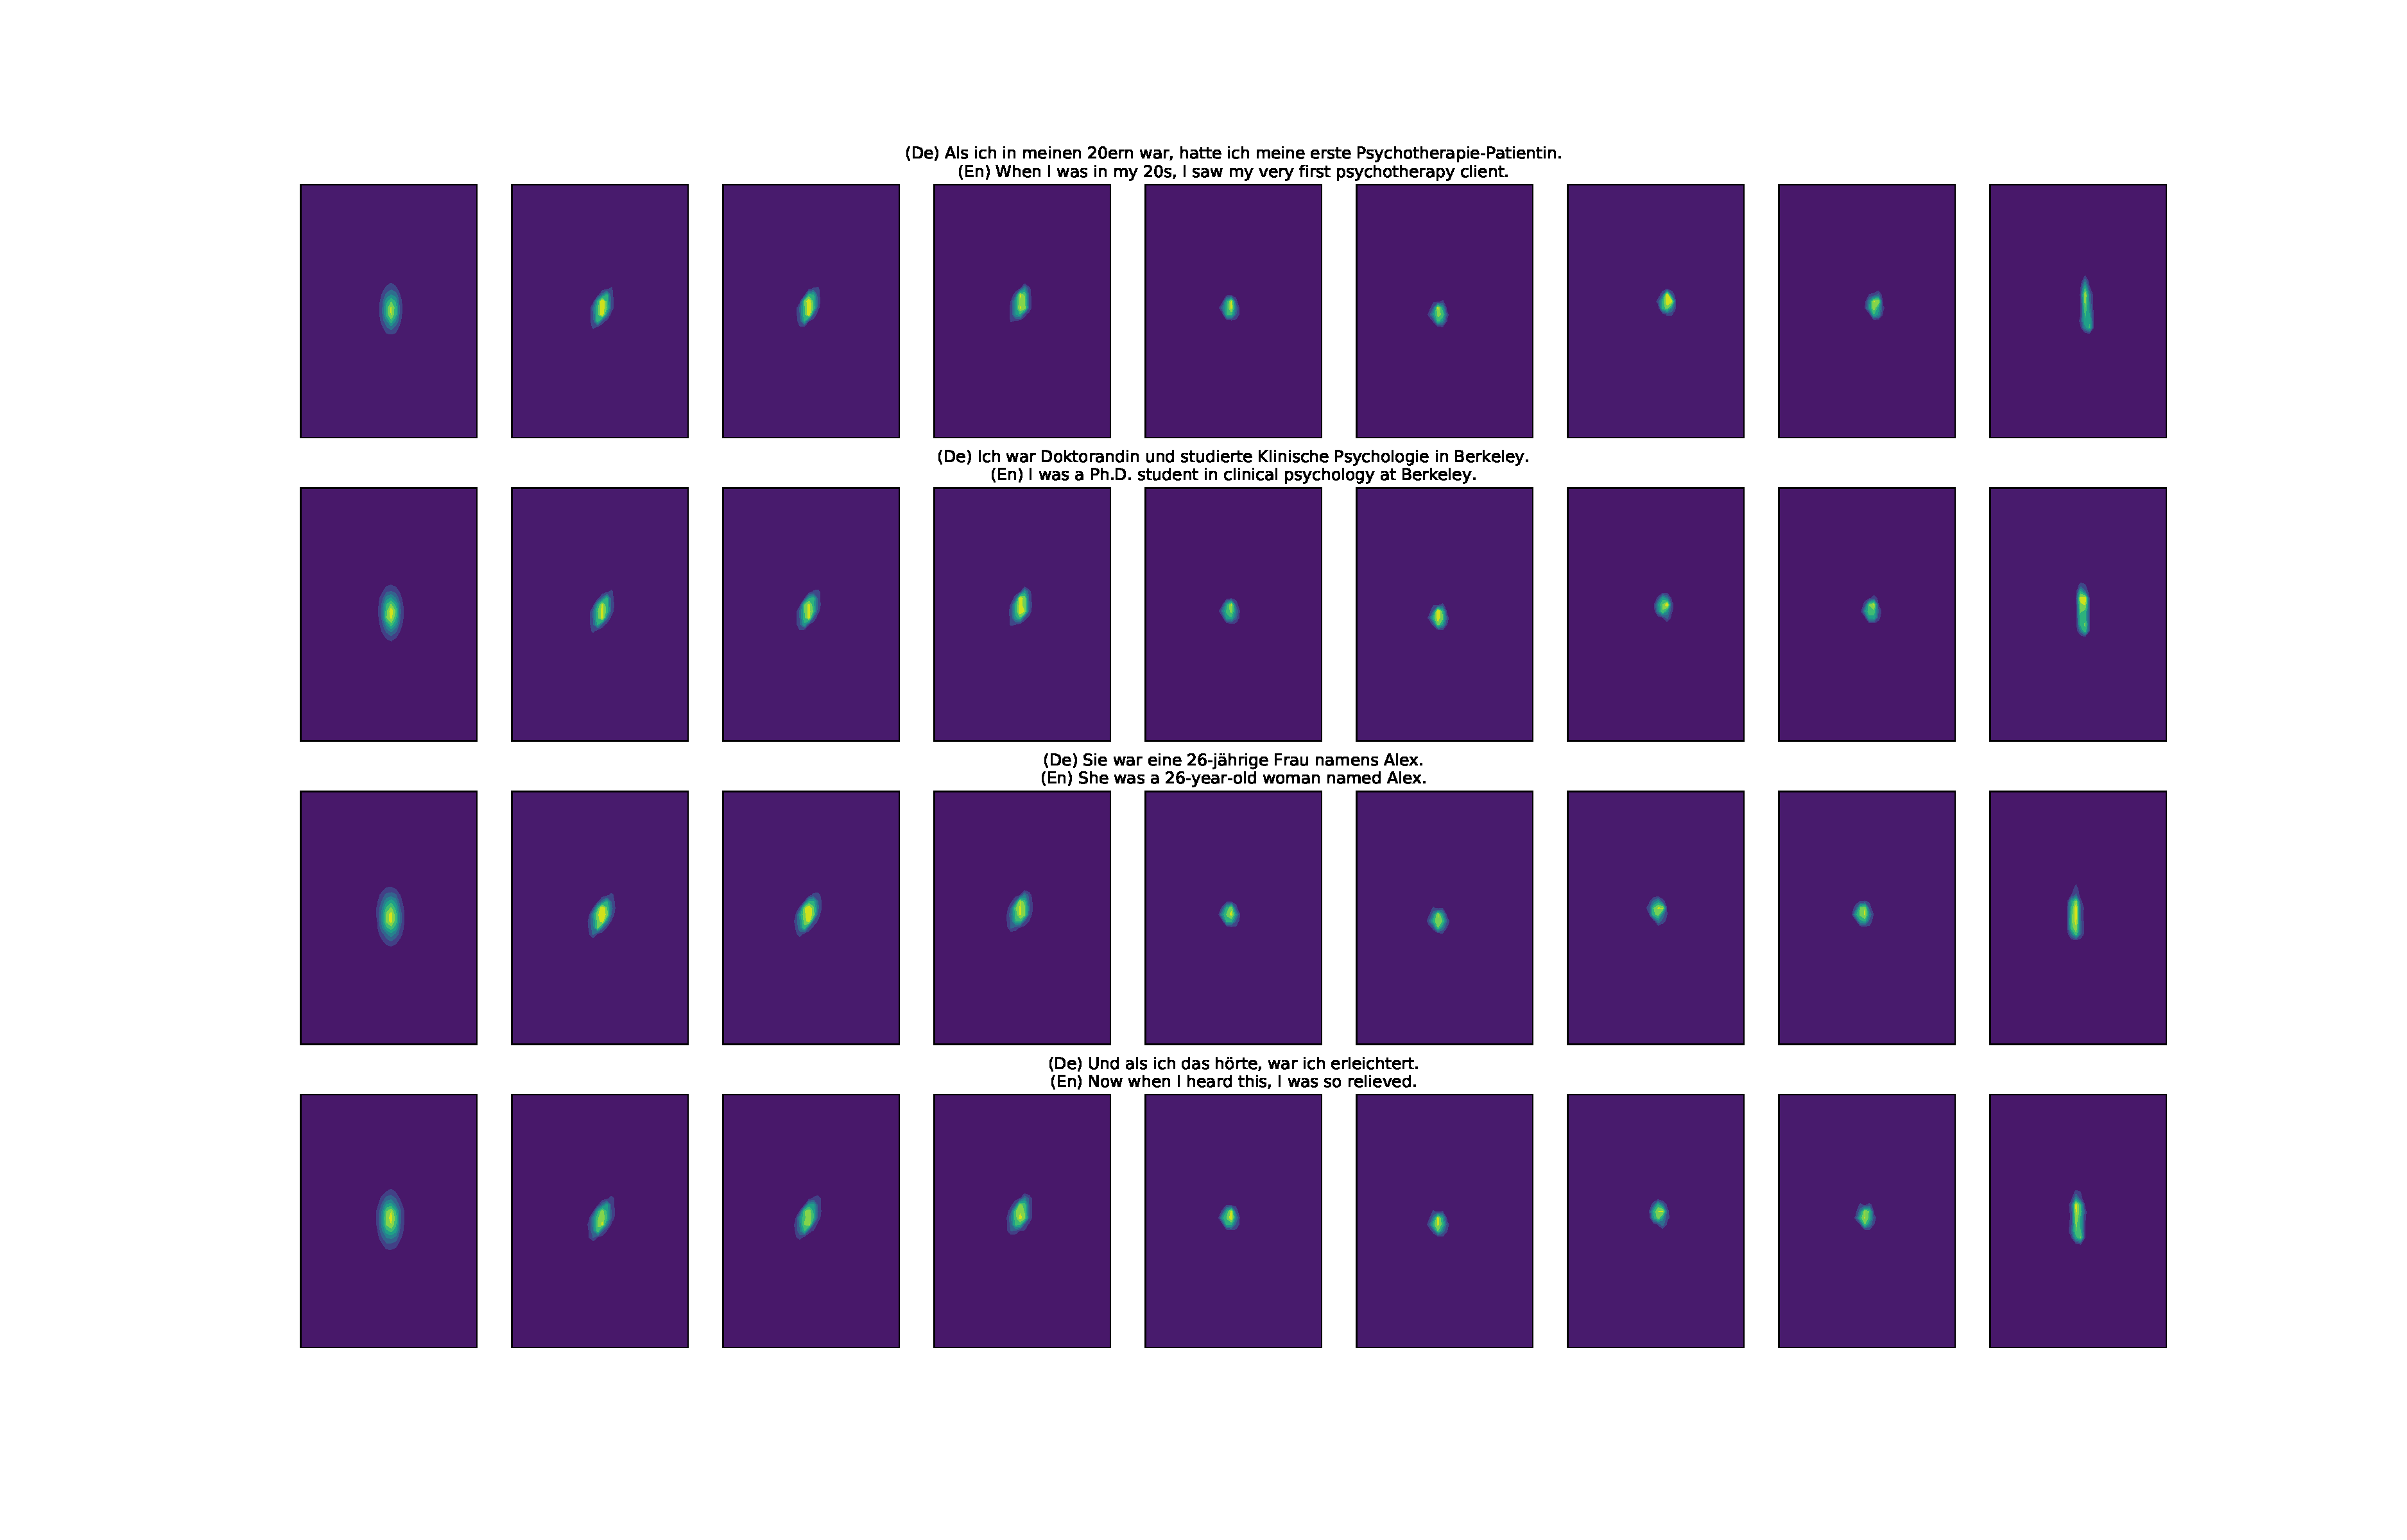
\includegraphics[width=\textwidth]{vaenmt_planar_flows_plot.pdf}
	\caption{One of our \ac{GNMT} models with 2 dimensional latent space, and 8 planar flows. Each row is a sentence pair with an increasing number of flows applied from 0 through 8. The ordering is 0 flows on the far left, and 8 flows on the far right. }
	\label{fig:gnmt_planar}
\end{figure}

\begin{figure}[b]{}
	\centering
	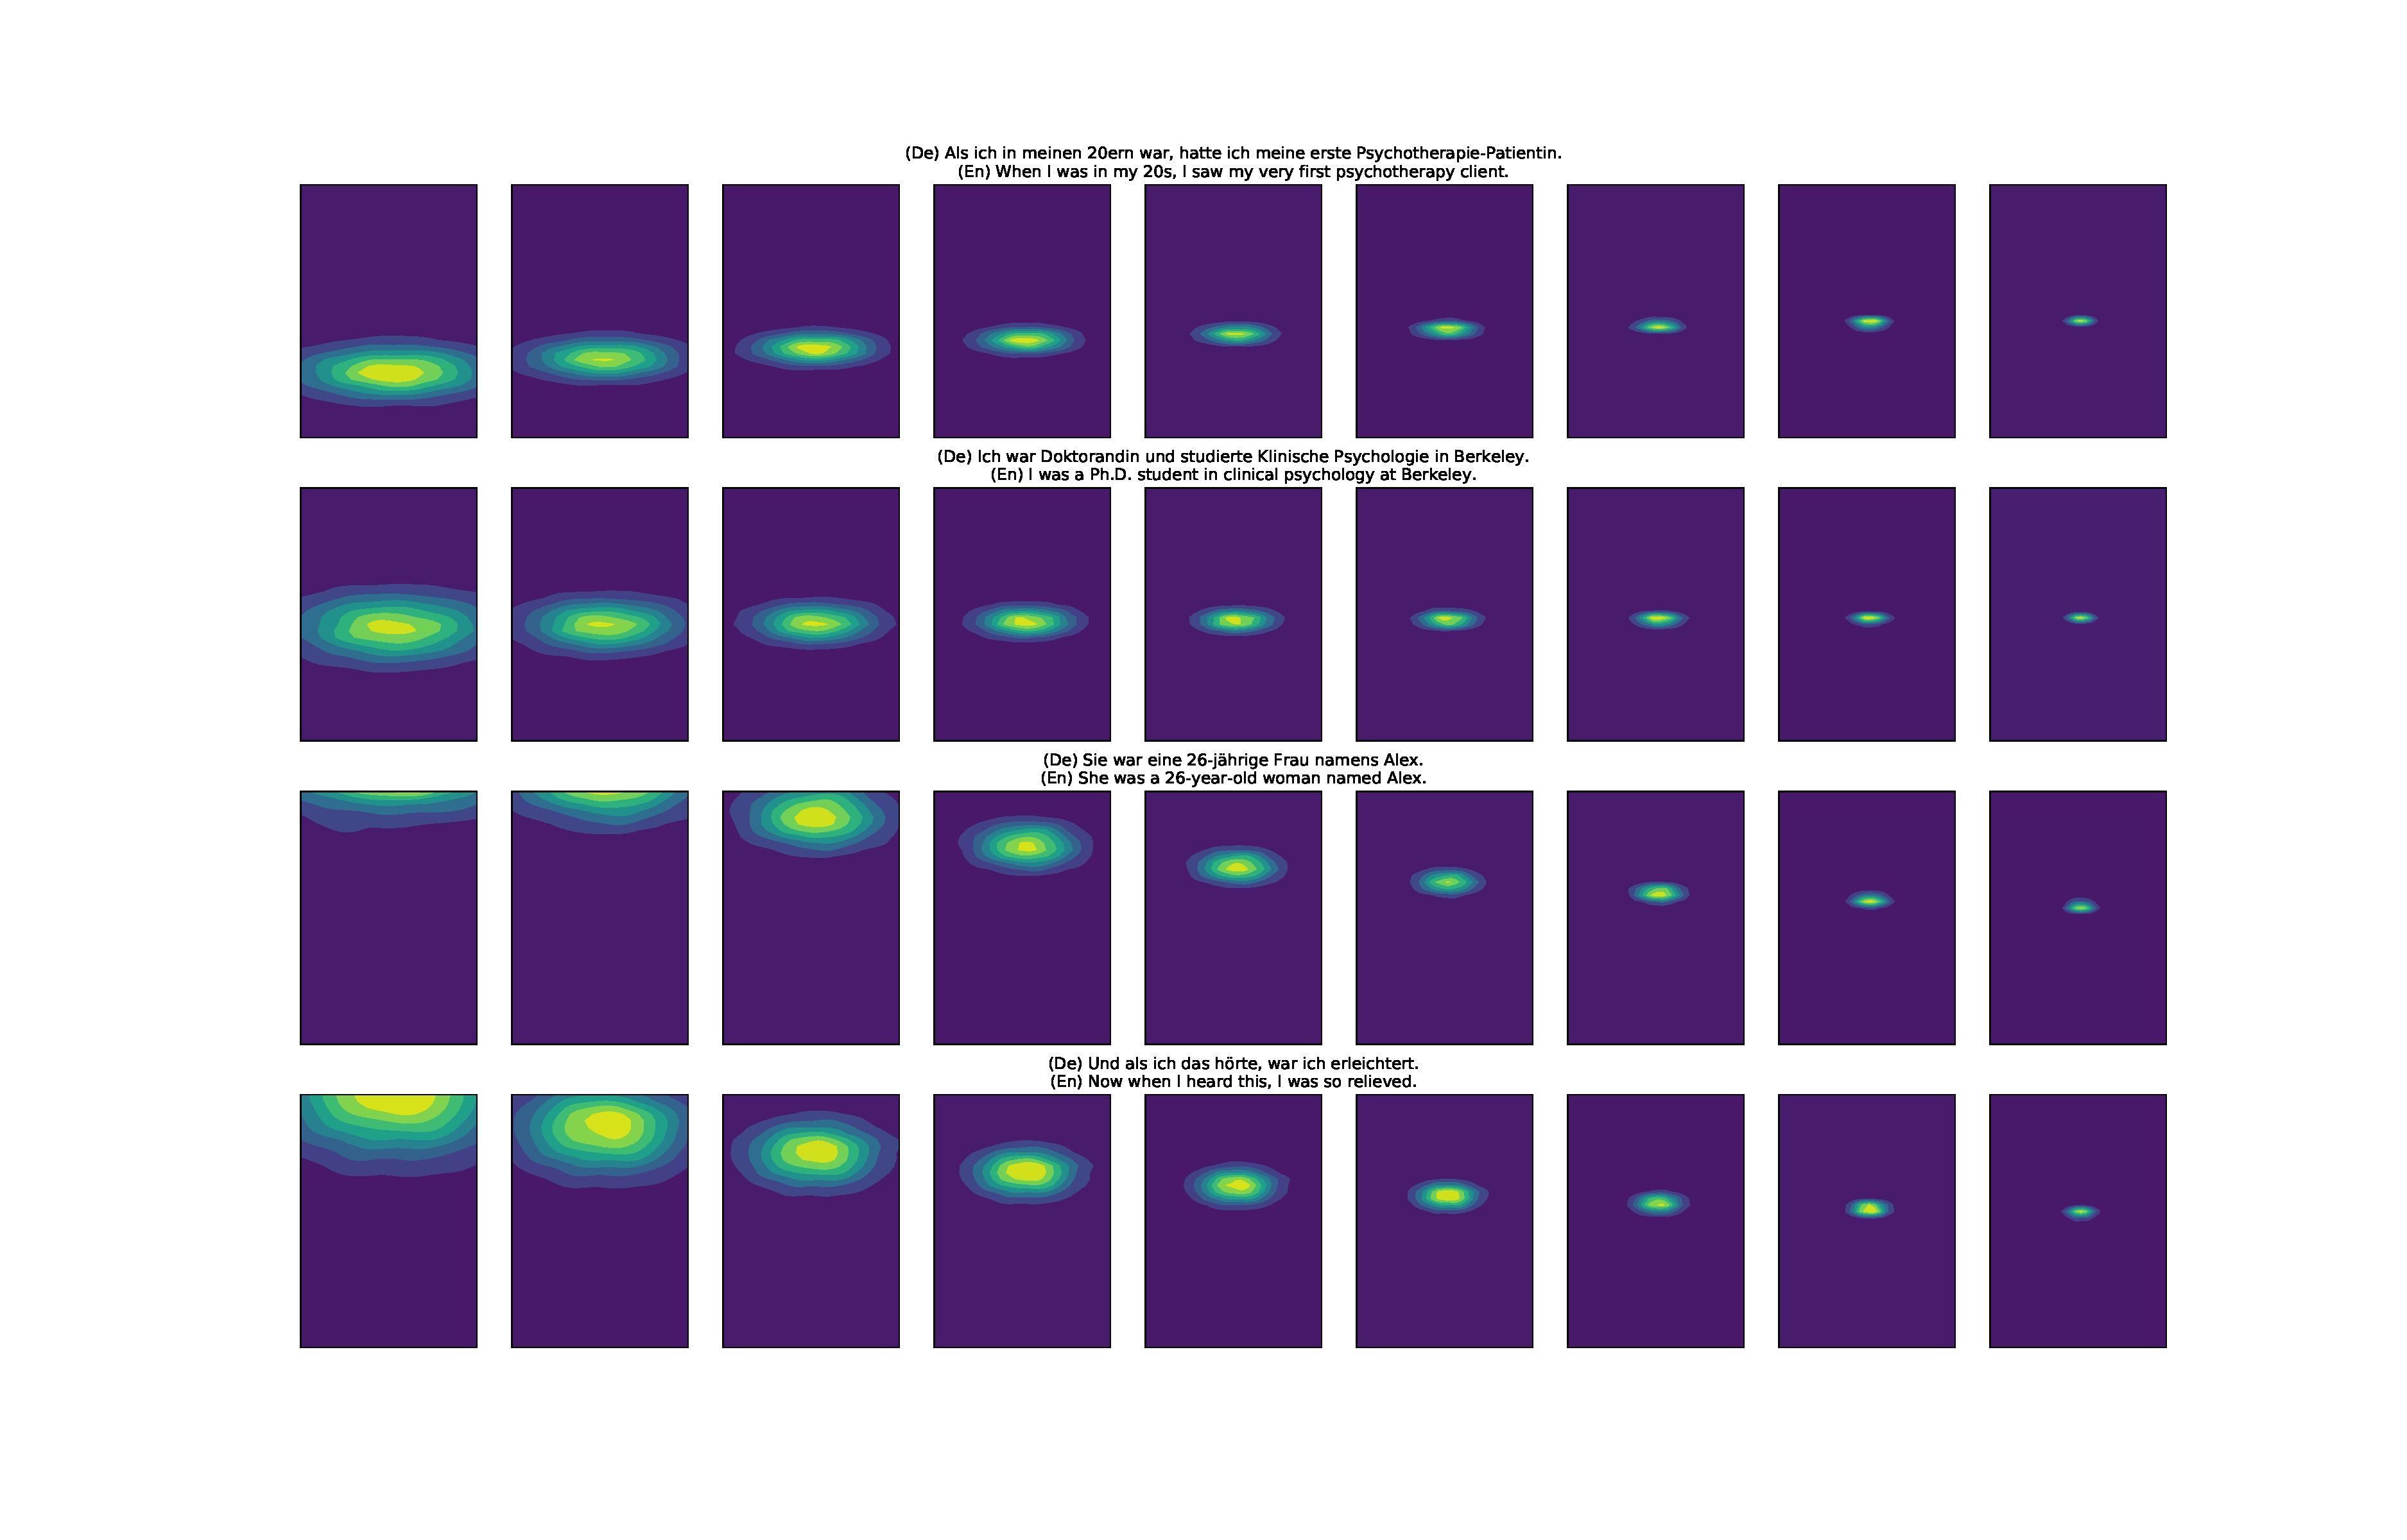
\includegraphics[width=\textwidth]{vaenmt_iaf_flows_plot.pdf}
	\caption{One of our 2 dimensional latent variable \ac{GNMT}  models trained with 8 \ac{IAF} flows. Each row is one sentence pair with an increasing number of flows applied to samples from the base distribution. Each row is a sentence pair with an increasing number of flows applied from 0 through 8. The ordering is 0 flows on the far left, and 8 flows on the far right.  }
	\label{fig:gnmt_iaf}
\end{figure}



\begin{figure}[b]{}
	\centering
	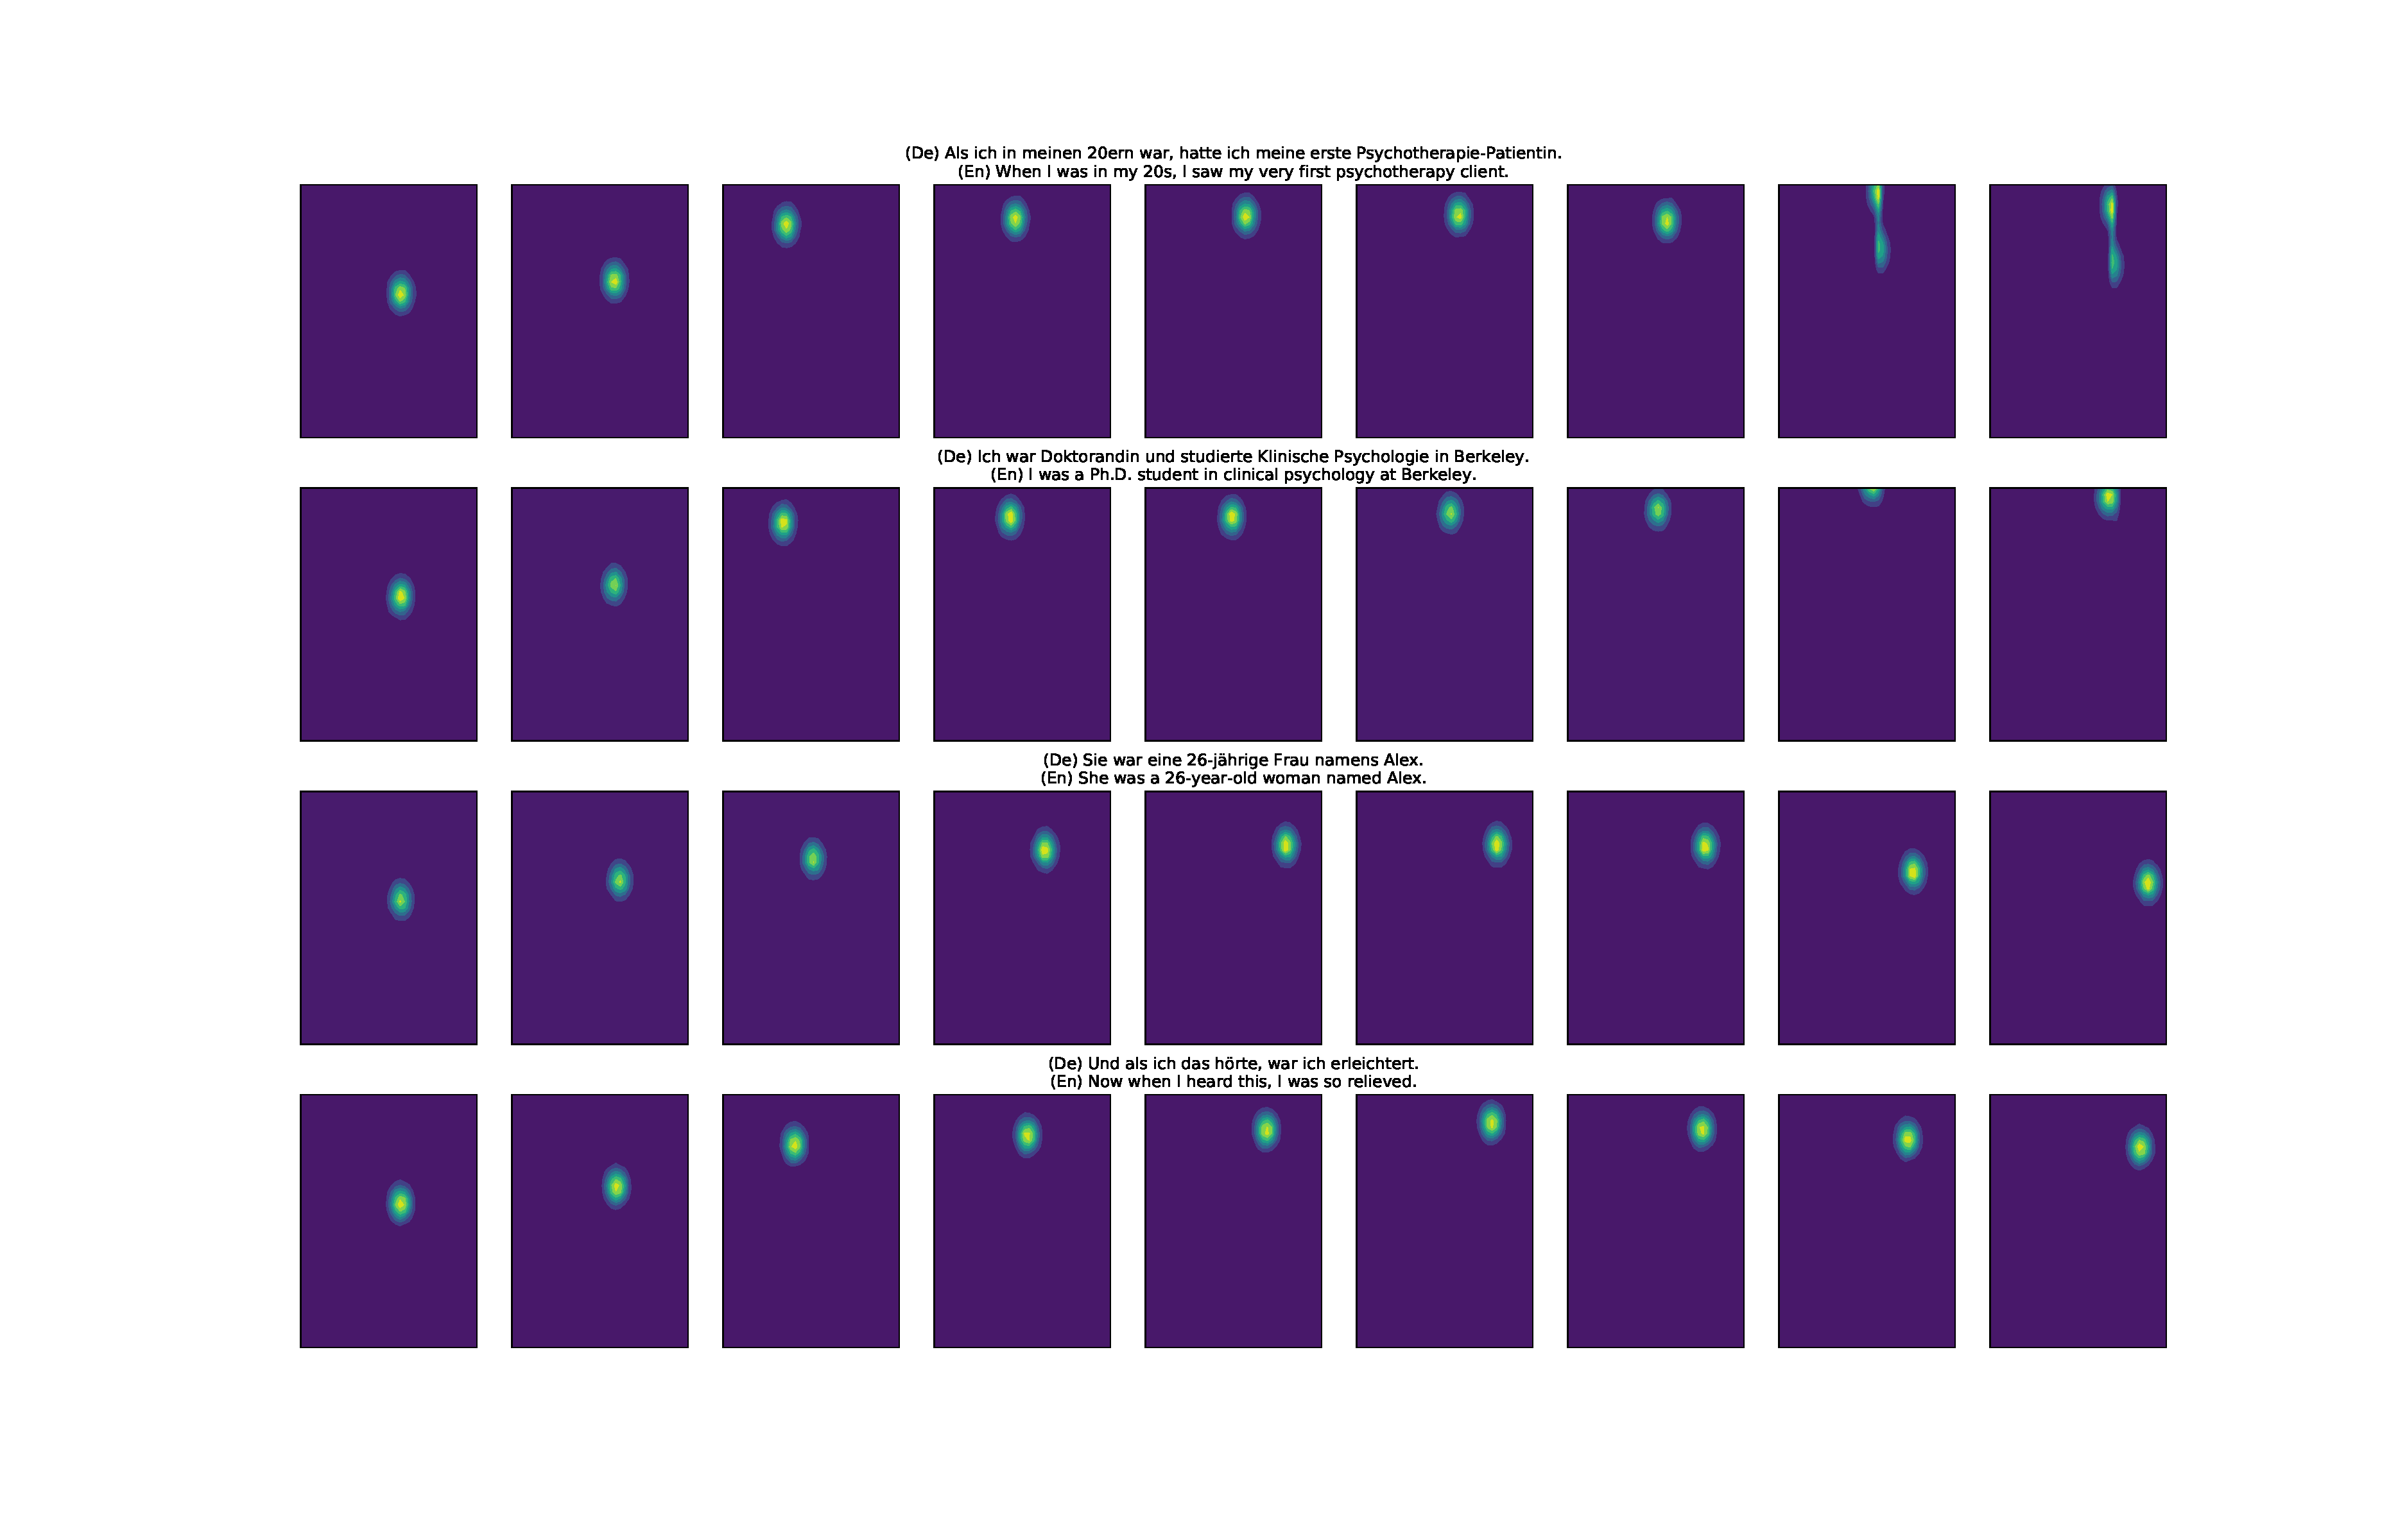
\includegraphics[width=\textwidth]{vnmt_planar_flows_plot.pdf}
	\caption{Two dimensional latent variable \ac{VNMT} with 8 planar flows. Captions are the sentence pairs. Each row is a sentence pair with an increasing number of flows applied from 0 through 8. The ordering is 0 flows on the far left, and 8 flows on the far right.  }
	\label{fig:vnmt_planar}
\end{figure}

\begin{figure}[b]{}
	\centering
	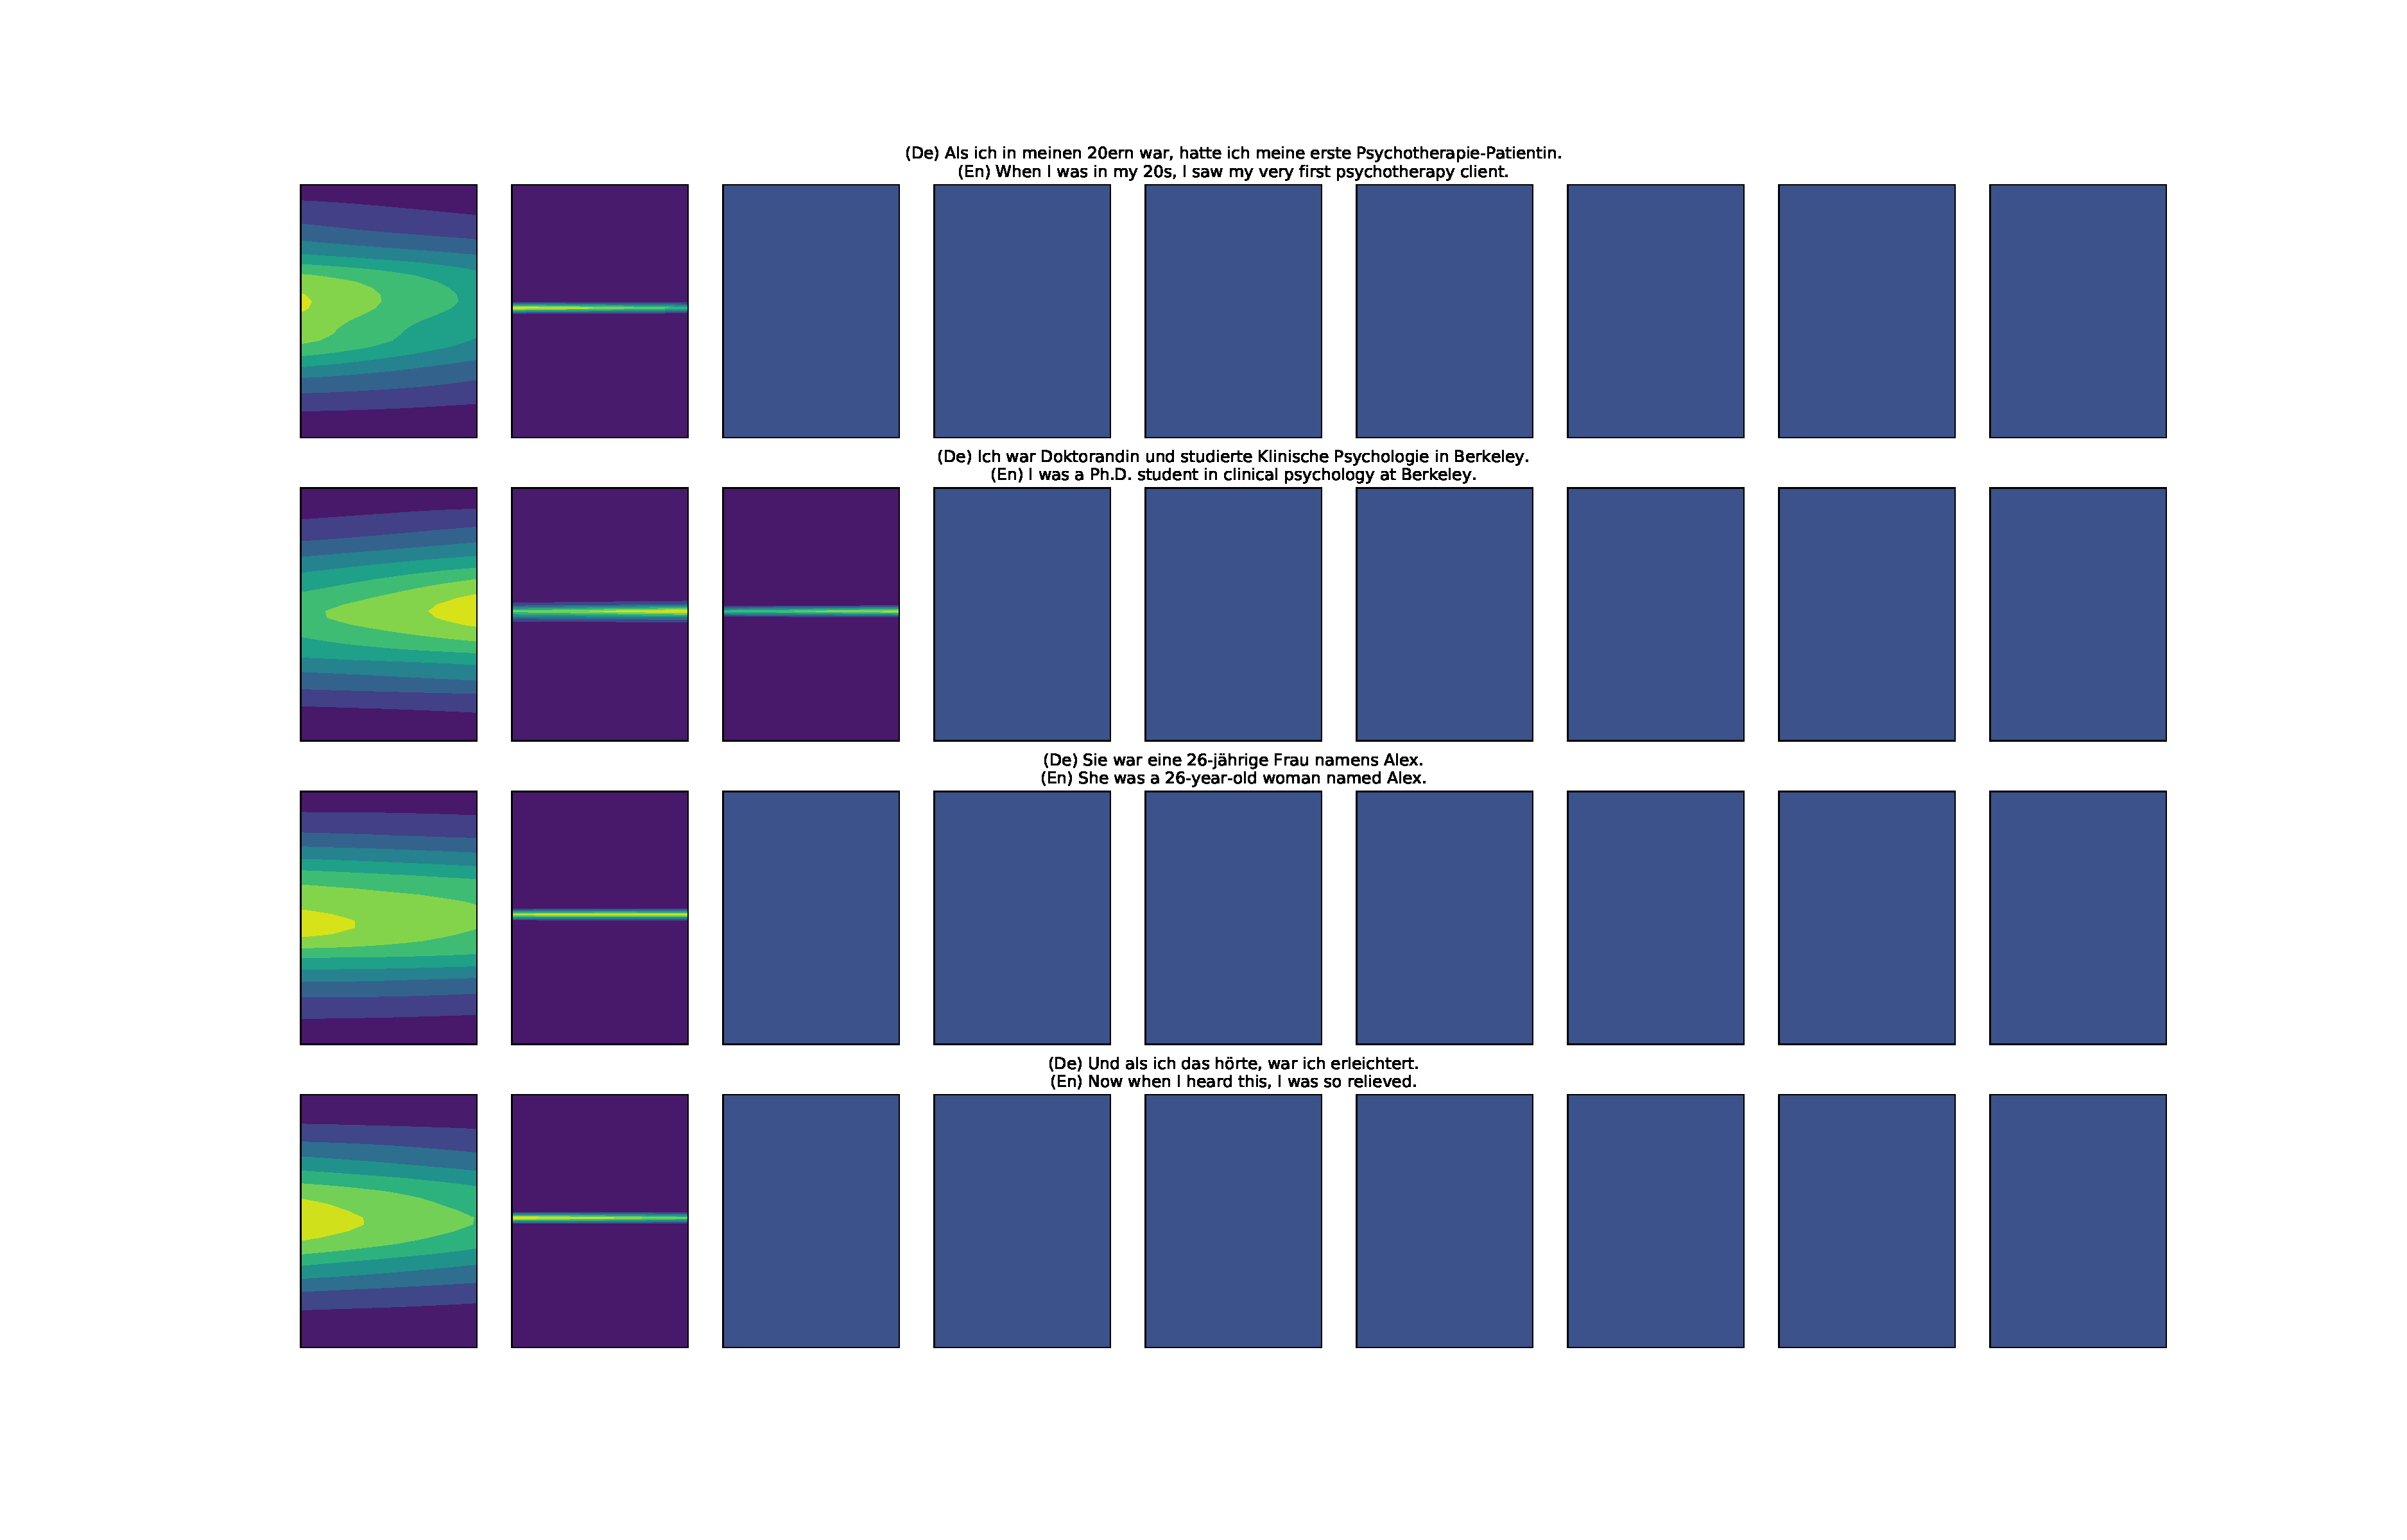
\includegraphics[width=\textwidth]{vnmt_iaf_flows_plot.pdf}
	\caption{Visualization of several sentence pairs latent spaces with \ac{VNMT} model and 8 \ac{IAF} flows. Solid blue images mean the distribution has been flattened into a line. Each row is a sentence pair with 0 flows on the far left and 8 flows applied on the right.  }
	\label{fig:vnmt_iaf}
\end{figure}



\begin{table}[]
	\caption{BLEU score difference of \ac{GNMT} with attention when language model is not optimized during training. We include \ac{GNMT} with language model training for reference. The comparison just shows that without the language model, \ac{GNMT} does not incorporate information at all from the latent variable $z$.  }
	\label{tab:de_en_vaenmt_bleu_no_lm_delta_bleu_sup}
	\center	
	\begin{tabular}{cccccccc}
		\multicolumn{8}{c}{\textbf{Latent Dimension: 128 (BLEU Difference)}}                                                                                                                                                                                                                                                                                                                                                                                                                              \\ \hline
		\multicolumn{1}{|c|}{\textbf{Flows}}                          & \multicolumn{1}{c|}{\textbf{1}}                   & \multicolumn{1}{c|}{\textbf{2}}                    & \multicolumn{1}{c|}{\textbf{4}}                    & \multicolumn{1}{c|}{\textbf{8}}                   & \multicolumn{1}{c|}{\textbf{16}}                   & \multicolumn{1}{c|}{\textbf{0 (Baseline)}}                          & \multicolumn{1}{c|}{\textbf{Model}}                                                  \\ \hline
		\rowcolor[HTML]{CEF2F1} 
		\multicolumn{1}{|c|}{\cellcolor[HTML]{CEF2F1}Planar}          & \multicolumn{1}{c|}{\cellcolor[HTML]{CEF2F1}0.0}  & \multicolumn{1}{c|}{\cellcolor[HTML]{CEF2F1}0.0}   & \multicolumn{1}{c|}{\cellcolor[HTML]{CEF2F1}0.0}   & \multicolumn{1}{c|}{\cellcolor[HTML]{CEF2F1}0.0}  & \multicolumn{1}{c|}{\cellcolor[HTML]{CEF2F1}0.0}   & \multicolumn{1}{c|}{\cellcolor[HTML]{CEF2F1}}                       & \multicolumn{1}{c|}{\cellcolor[HTML]{CEF2F1}}                                        \\ \cline{1-6}
		\rowcolor[HTML]{CEF2F1} 
		\multicolumn{1}{|c|}{\cellcolor[HTML]{CEF2F1}IAF}             & \multicolumn{1}{c|}{\cellcolor[HTML]{CEF2F1}0.0}  & \multicolumn{1}{c|}{\cellcolor[HTML]{CEF2F1}0.0}   & \multicolumn{1}{c|}{\cellcolor[HTML]{CEF2F1}0.0}   & \multicolumn{1}{c|}{\cellcolor[HTML]{CEF2F1}0.0}  & \multicolumn{1}{c|}{\cellcolor[HTML]{CEF2F1}0.0}   & \multicolumn{1}{c|}{\multirow{-2}{*}{\cellcolor[HTML]{CEF2F1}0.0}}  & \multicolumn{1}{c|}{\multirow{-2}{*}{\cellcolor[HTML]{CEF2F1}GNMT (No LM)}}          \\ \hline
		\rowcolor[HTML]{F4DAD8} 
		\multicolumn{1}{|c|}{\cellcolor[HTML]{F4DAD8}Planar}          & \multicolumn{1}{c|}{\cellcolor[HTML]{F4DAD8}0.14} & \multicolumn{1}{c|}{\cellcolor[HTML]{F4DAD8}0.08}  & \multicolumn{1}{c|}{\cellcolor[HTML]{F4DAD8}0.02}  & \multicolumn{1}{c|}{\cellcolor[HTML]{F4DAD8}0.06} & \multicolumn{1}{c|}{\cellcolor[HTML]{F4DAD8}0.1}   & \multicolumn{1}{c|}{\cellcolor[HTML]{F4DAD8}}                       & \multicolumn{1}{c|}{\cellcolor[HTML]{F4DAD8}}                                        \\ \cline{1-6}
		\rowcolor[HTML]{F4DAD8} 
		\multicolumn{1}{|c|}{\cellcolor[HTML]{F4DAD8}IAF}             & \multicolumn{1}{c|}{\cellcolor[HTML]{F4DAD8}0.12} & \multicolumn{1}{c|}{\cellcolor[HTML]{F4DAD8}0.08}  & \multicolumn{1}{c|}{\cellcolor[HTML]{F4DAD8}-0.01} & \multicolumn{1}{c|}{\cellcolor[HTML]{F4DAD8}0.1}  & \multicolumn{1}{c|}{\cellcolor[HTML]{F4DAD8}-0.01} & \multicolumn{1}{c|}{\multirow{-2}{*}{\cellcolor[HTML]{F4DAD8}0.08}} & \multicolumn{1}{c|}{\multirow{-2}{*}{\cellcolor[HTML]{F4DAD8}GNMT}}                  \\ \hline
		\multicolumn{8}{c}{\textbf{Latent Dimension: 256  (BLEU Difference)}}                                                                                                                                                                                                                                                                                                                                                                                                                             \\ \hline
		\multicolumn{1}{|c|}{\textbf{Flows}}                          & \multicolumn{1}{c|}{\textbf{1}}                   & \multicolumn{1}{c|}{\textbf{2}}                    & \multicolumn{1}{c|}{\textbf{4}}                    & \multicolumn{1}{c|}{\textbf{8}}                   & \multicolumn{1}{c|}{\textbf{16}}                   & \multicolumn{1}{c|}{\textbf{0 (Baseline)}}                          & \multicolumn{1}{c|}{\textbf{Model}}                                                  \\ \hline
		\rowcolor[HTML]{CEF2F1} 
		\multicolumn{1}{|c|}{\cellcolor[HTML]{CEF2F1}Planar} & \multicolumn{1}{c|}{\cellcolor[HTML]{CEF2F1}0.0}  & \multicolumn{1}{c|}{\cellcolor[HTML]{CEF2F1}0.0}   & \multicolumn{1}{c|}{\cellcolor[HTML]{CEF2F1}0.0}   & \multicolumn{1}{c|}{\cellcolor[HTML]{CEF2F1}0.0}  & \multicolumn{1}{c|}{\cellcolor[HTML]{CEF2F1}0.0}   & \multicolumn{1}{c|}{\cellcolor[HTML]{CEF2F1}}                       & \multicolumn{1}{c|}{\cellcolor[HTML]{CEF2F1}}                                        \\ \cline{1-6}
		\rowcolor[HTML]{CEF2F1} 
		\multicolumn{1}{|c|}{\cellcolor[HTML]{CEF2F1}IAF}    & \multicolumn{1}{c|}{\cellcolor[HTML]{CEF2F1}0.0}  & \multicolumn{1}{c|}{\cellcolor[HTML]{CEF2F1}0.0}   & \multicolumn{1}{c|}{\cellcolor[HTML]{CEF2F1}0.0}   & \multicolumn{1}{c|}{\cellcolor[HTML]{CEF2F1}0.0}  & \multicolumn{1}{c|}{\cellcolor[HTML]{CEF2F1}0.0}   & \multicolumn{1}{c|}{\multirow{-2}{*}{\cellcolor[HTML]{CEF2F1}0.0}}  & \multicolumn{1}{c|}{\multirow{-2}{*}{\cellcolor[HTML]{CEF2F1}GNMT (No LM)}} \\ \hline
		\rowcolor[HTML]{F4DAD8} 
		\multicolumn{1}{|c|}{\cellcolor[HTML]{F4DAD8}Planar}          & \multicolumn{1}{c|}{\cellcolor[HTML]{F4DAD8}0.1}  & \multicolumn{1}{c|}{\cellcolor[HTML]{F4DAD8}0}     & \multicolumn{1}{c|}{\cellcolor[HTML]{F4DAD8}0.11}  & \multicolumn{1}{c|}{\cellcolor[HTML]{F4DAD8}0.15} & \multicolumn{1}{c|}{\cellcolor[HTML]{F4DAD8}0.04}  & \multicolumn{1}{c|}{\cellcolor[HTML]{F4DAD8}}                       & \multicolumn{1}{c|}{\cellcolor[HTML]{F4DAD8}}                                        \\ \cline{1-6}
		\rowcolor[HTML]{F4DAD8} 
		\multicolumn{1}{|c|}{\cellcolor[HTML]{F4DAD8}IAF}             & \multicolumn{1}{c|}{\cellcolor[HTML]{F4DAD8}0.04} & \multicolumn{1}{c|}{\cellcolor[HTML]{F4DAD8}0.09}  & \multicolumn{1}{c|}{\cellcolor[HTML]{F4DAD8}0.04}  & \multicolumn{1}{c|}{\cellcolor[HTML]{F4DAD8}0.06} & \multicolumn{1}{c|}{\cellcolor[HTML]{F4DAD8}0.19}  & \multicolumn{1}{c|}{\multirow{-2}{*}{\cellcolor[HTML]{F4DAD8}0.09}} & \multicolumn{1}{c|}{\multirow{-2}{*}{\cellcolor[HTML]{F4DAD8}GNMT}}                  \\ \hline
	\end{tabular}
\end{table}


% some may be copies of above


\begin{table}[]
	\label{tab:no_attn_no_lm_kl_divergence}
	\caption{KL divergence for \ac{GNMT} models trained without attention or language model optimization. Results suggest posterior collapse has occurred as the values are almost all near 0. }
	\center
	\begin{tabular}{cccccccc}
		\multicolumn{8}{c}{\textbf{Latent Dimension: 128 (KL Divergence)}}                                                                                                                                                                                                                                                                                                                                                                                                           \\ \hline
		\multicolumn{1}{|c|}{\textbf{Flows}}                 & \multicolumn{1}{c|}{\textbf{1}}                   & \multicolumn{1}{c|}{\textbf{2}}                   & \multicolumn{1}{c|}{\textbf{4}}                   & \multicolumn{1}{c|}{\textbf{8}}                   & \multicolumn{1}{c|}{\textbf{16}}                  & \multicolumn{1}{c|}{\textbf{0 (Baseline)}}                          & \multicolumn{1}{c|}{\textbf{Model}}                                         \\ \hline
		\rowcolor[HTML]{CEF2F1} 
		\multicolumn{1}{|c|}{\cellcolor[HTML]{CEF2F1}Planar} & \multicolumn{1}{c|}{\cellcolor[HTML]{CEF2F1}0.0}  & \multicolumn{1}{c|}{\cellcolor[HTML]{CEF2F1}0.0}  & \multicolumn{1}{c|}{\cellcolor[HTML]{CEF2F1}0.0}  & \multicolumn{1}{c|}{\cellcolor[HTML]{CEF2F1}0.01} & \multicolumn{1}{c|}{\cellcolor[HTML]{CEF2F1}0.01} & \multicolumn{1}{c|}{\cellcolor[HTML]{CEF2F1}}                       & \multicolumn{1}{c|}{\cellcolor[HTML]{CEF2F1}}                               \\ \cline{1-6}
		\rowcolor[HTML]{CEF2F1} 
		\multicolumn{1}{|c|}{\cellcolor[HTML]{CEF2F1}IAF}    & \multicolumn{1}{c|}{\cellcolor[HTML]{CEF2F1}0.0}  & \multicolumn{1}{c|}{\cellcolor[HTML]{CEF2F1}0.0}  & \multicolumn{1}{c|}{\cellcolor[HTML]{CEF2F1}0.01} & \multicolumn{1}{c|}{\cellcolor[HTML]{CEF2F1}0.0}  & \multicolumn{1}{c|}{\cellcolor[HTML]{CEF2F1}0.0}  & \multicolumn{1}{c|}{\multirow{-2}{*}{\cellcolor[HTML]{CEF2F1}0.0}}  & \multicolumn{1}{c|}{\multirow{-2}{*}{\cellcolor[HTML]{CEF2F1}GNMT (No LM)}} \\ \hline
		\rowcolor[HTML]{F4DAD8} 
		\multicolumn{1}{|c|}{\cellcolor[HTML]{F4DAD8}Planar} & \multicolumn{1}{c|}{\cellcolor[HTML]{F4DAD8}4.28} & \multicolumn{1}{c|}{\cellcolor[HTML]{F4DAD8}4.48} & \multicolumn{1}{c|}{\cellcolor[HTML]{F4DAD8}3.84} & \multicolumn{1}{c|}{\cellcolor[HTML]{F4DAD8}4.12} & \multicolumn{1}{c|}{\cellcolor[HTML]{F4DAD8}4.58} & \multicolumn{1}{c|}{\cellcolor[HTML]{F4DAD8}}                       & \multicolumn{1}{c|}{\cellcolor[HTML]{F4DAD8}}                               \\ \cline{1-6}
		\rowcolor[HTML]{F4DAD8} 
		\multicolumn{1}{|c|}{\cellcolor[HTML]{F4DAD8}IAF}    & \multicolumn{1}{c|}{\cellcolor[HTML]{F4DAD8}3.38} & \multicolumn{1}{c|}{\cellcolor[HTML]{F4DAD8}2.97} & \multicolumn{1}{c|}{\cellcolor[HTML]{F4DAD8}3.89} & \multicolumn{1}{c|}{\cellcolor[HTML]{F4DAD8}4.57} & \multicolumn{1}{c|}{\cellcolor[HTML]{F4DAD8}4.53} & \multicolumn{1}{c|}{\multirow{-2}{*}{\cellcolor[HTML]{F4DAD8}2.23}} & \multicolumn{1}{c|}{\multirow{-2}{*}{\cellcolor[HTML]{F4DAD8}GNMT}}         \\ \hline
		\multicolumn{8}{c}{\textbf{Latent Dimension: 256 (KL Divergence)}}                                                                                                                                                                                                                                                                                                                                                                                                           \\ \hline
		\multicolumn{1}{|c|}{\textbf{Flows}}                 & \multicolumn{1}{c|}{\textbf{1}}                   & \multicolumn{1}{c|}{\textbf{2}}                   & \multicolumn{1}{c|}{\textbf{4}}                   & \multicolumn{1}{c|}{\textbf{8}}                   & \multicolumn{1}{c|}{\textbf{16}}                  & \multicolumn{1}{c|}{\textbf{0 (Baseline)}}                          & \multicolumn{1}{c|}{\textbf{Model}}                                         \\ \hline
		\rowcolor[HTML]{CEF2F1} 
		\multicolumn{1}{|c|}{\cellcolor[HTML]{CEF2F1}Planar} & \multicolumn{1}{c|}{\cellcolor[HTML]{CEF2F1}0.01} & \multicolumn{1}{c|}{\cellcolor[HTML]{CEF2F1}0.01} & \multicolumn{1}{c|}{\cellcolor[HTML]{CEF2F1}0.01} & \multicolumn{1}{c|}{\cellcolor[HTML]{CEF2F1}0.01} & \multicolumn{1}{c|}{\cellcolor[HTML]{CEF2F1}0.02} & \multicolumn{1}{c|}{\cellcolor[HTML]{CEF2F1}}                       & \multicolumn{1}{c|}{\cellcolor[HTML]{CEF2F1}}                               \\ \cline{1-6}
		\rowcolor[HTML]{CEF2F1} 
		\multicolumn{1}{|c|}{\cellcolor[HTML]{CEF2F1}IAF}    & \multicolumn{1}{c|}{\cellcolor[HTML]{CEF2F1}0.01} & \multicolumn{1}{c|}{\cellcolor[HTML]{CEF2F1}0.01} & \multicolumn{1}{c|}{\cellcolor[HTML]{CEF2F1}0.01} & \multicolumn{1}{c|}{\cellcolor[HTML]{CEF2F1}0.01} & \multicolumn{1}{c|}{\cellcolor[HTML]{CEF2F1}0.01} & \multicolumn{1}{c|}{\multirow{-2}{*}{\cellcolor[HTML]{CEF2F1}0.0}}  & \multicolumn{1}{c|}{\multirow{-2}{*}{\cellcolor[HTML]{CEF2F1}GNMT (No LM)}} \\ \hline
		\rowcolor[HTML]{F4DAD8} 
		\multicolumn{1}{|c|}{\cellcolor[HTML]{F4DAD8}Planar} & \multicolumn{1}{c|}{\cellcolor[HTML]{F4DAD8}4.1}  & \multicolumn{1}{c|}{\cellcolor[HTML]{F4DAD8}4.26} & \multicolumn{1}{c|}{\cellcolor[HTML]{F4DAD8}3.57} & \multicolumn{1}{c|}{\cellcolor[HTML]{F4DAD8}3.54} & \multicolumn{1}{c|}{\cellcolor[HTML]{F4DAD8}3.65} & \multicolumn{1}{c|}{\cellcolor[HTML]{F4DAD8}}                       & \multicolumn{1}{c|}{\cellcolor[HTML]{F4DAD8}}                               \\ \cline{1-6}
		\rowcolor[HTML]{F4DAD8} 
		\multicolumn{1}{|c|}{\cellcolor[HTML]{F4DAD8}IAF}    & \multicolumn{1}{c|}{\cellcolor[HTML]{F4DAD8}3.99} & \multicolumn{1}{c|}{\cellcolor[HTML]{F4DAD8}3.19} & \multicolumn{1}{c|}{\cellcolor[HTML]{F4DAD8}3.99} & \multicolumn{1}{c|}{\cellcolor[HTML]{F4DAD8}3.12} & \multicolumn{1}{c|}{\cellcolor[HTML]{F4DAD8}3.45} & \multicolumn{1}{c|}{\multirow{-2}{*}{\cellcolor[HTML]{F4DAD8}4.19}} & \multicolumn{1}{c|}{\multirow{-2}{*}{\cellcolor[HTML]{F4DAD8}GNMT}}         \\ \hline
	\end{tabular}
\end{table}

\begin{table}[]
	\label{tab:no_attn_no_lm_bleu_diff}
	\caption{ Measure of performance drop when $z$ is removed from trained system for \ac{GNMT} without attention or  language model  optimization. }	
	\center
	\begin{tabular}{cccccccc}
		\multicolumn{8}{c}{\textbf{Latent Dimension: 128 (BLEU Difference)}}                                                                                                                                                                                                                                                                                                                                                                                                         \\ \hline
		\multicolumn{1}{|c|}{\textbf{Flows}}                 & \multicolumn{1}{c|}{\textbf{1}}                   & \multicolumn{1}{c|}{\textbf{2}}                   & \multicolumn{1}{c|}{\textbf{4}}                   & \multicolumn{1}{c|}{\textbf{8}}                   & \multicolumn{1}{c|}{\textbf{16}}                  & \multicolumn{1}{c|}{\textbf{0 (Baseline)}}                          & \multicolumn{1}{c|}{\textbf{Model}}                                         \\ \hline
		\rowcolor[HTML]{CEF2F1} 
		\multicolumn{1}{|c|}{\cellcolor[HTML]{CEF2F1}Planar} & \multicolumn{1}{c|}{\cellcolor[HTML]{CEF2F1}0.0}  & \multicolumn{1}{c|}{\cellcolor[HTML]{CEF2F1}0.0}  & \multicolumn{1}{c|}{\cellcolor[HTML]{CEF2F1}0.0}  & \multicolumn{1}{c|}{\cellcolor[HTML]{CEF2F1}0.0}  & \multicolumn{1}{c|}{\cellcolor[HTML]{CEF2F1}0.0}  & \multicolumn{1}{c|}{\cellcolor[HTML]{CEF2F1}}                       & \multicolumn{1}{c|}{\cellcolor[HTML]{CEF2F1}}                               \\ \cline{1-6}
		\rowcolor[HTML]{CEF2F1} 
		\multicolumn{1}{|c|}{\cellcolor[HTML]{CEF2F1}IAF}    & \multicolumn{1}{c|}{\cellcolor[HTML]{CEF2F1}0.0}  & \multicolumn{1}{c|}{\cellcolor[HTML]{CEF2F1}0.0}  & \multicolumn{1}{c|}{\cellcolor[HTML]{CEF2F1}0.0}  & \multicolumn{1}{c|}{\cellcolor[HTML]{CEF2F1}0.0}  & \multicolumn{1}{c|}{\cellcolor[HTML]{CEF2F1}0.0}  & \multicolumn{1}{c|}{\multirow{-2}{*}{\cellcolor[HTML]{CEF2F1}0.0}}  & \multicolumn{1}{c|}{\multirow{-2}{*}{\cellcolor[HTML]{CEF2F1}GNMT (No LM)}} \\ \hline
		\rowcolor[HTML]{F4DAD8} 
		\multicolumn{1}{|c|}{\cellcolor[HTML]{F4DAD8}Planar} & \multicolumn{1}{c|}{\cellcolor[HTML]{F4DAD8}0.91} & \multicolumn{1}{c|}{\cellcolor[HTML]{F4DAD8}0.93} & \multicolumn{1}{c|}{\cellcolor[HTML]{F4DAD8}0.7}  & \multicolumn{1}{c|}{\cellcolor[HTML]{F4DAD8}0.49} & \multicolumn{1}{c|}{\cellcolor[HTML]{F4DAD8}0.72} & \multicolumn{1}{c|}{\cellcolor[HTML]{F4DAD8}}                       & \multicolumn{1}{c|}{\cellcolor[HTML]{F4DAD8}}                               \\ \cline{1-6}
		\rowcolor[HTML]{F4DAD8} 
		\multicolumn{1}{|c|}{\cellcolor[HTML]{F4DAD8}IAF}    & \multicolumn{1}{c|}{\cellcolor[HTML]{F4DAD8}0.88} & \multicolumn{1}{c|}{\cellcolor[HTML]{F4DAD8}0.59} & \multicolumn{1}{c|}{\cellcolor[HTML]{F4DAD8}0.88} & \multicolumn{1}{c|}{\cellcolor[HTML]{F4DAD8}0.79} & \multicolumn{1}{c|}{\cellcolor[HTML]{F4DAD8}1.1}  & \multicolumn{1}{c|}{\multirow{-2}{*}{\cellcolor[HTML]{F4DAD8}0.46}} & \multicolumn{1}{c|}{\multirow{-2}{*}{\cellcolor[HTML]{F4DAD8}GNMT}}         \\ \hline
		\multicolumn{8}{c}{\textbf{Latent Dimension: 256 (BLEU Difference)}}                                                                                                                                                                                                                                                                                                                                                                                                         \\ \hline
		\multicolumn{1}{|c|}{\textbf{Flows}}                 & \multicolumn{1}{c|}{\textbf{1}}                   & \multicolumn{1}{c|}{\textbf{2}}                   & \multicolumn{1}{c|}{\textbf{4}}                   & \multicolumn{1}{c|}{\textbf{8}}                   & \multicolumn{1}{c|}{\textbf{16}}                  & \multicolumn{1}{c|}{\textbf{0 (Baseline)}}                          & \multicolumn{1}{c|}{\textbf{Model}}                                         \\ \hline
		\rowcolor[HTML]{CEF2F1} 
		\multicolumn{1}{|c|}{\cellcolor[HTML]{CEF2F1}Planar} & \multicolumn{1}{c|}{\cellcolor[HTML]{CEF2F1}0.0}  & \multicolumn{1}{c|}{\cellcolor[HTML]{CEF2F1}0.0}  & \multicolumn{1}{c|}{\cellcolor[HTML]{CEF2F1}0.0}  & \multicolumn{1}{c|}{\cellcolor[HTML]{CEF2F1}0.0}  & \multicolumn{1}{c|}{\cellcolor[HTML]{CEF2F1}0.0}  & \multicolumn{1}{c|}{\cellcolor[HTML]{CEF2F1}}                       & \multicolumn{1}{c|}{\cellcolor[HTML]{CEF2F1}}                               \\ \cline{1-6}
		\rowcolor[HTML]{CEF2F1} 
		\multicolumn{1}{|c|}{\cellcolor[HTML]{CEF2F1}IAF}    & \multicolumn{1}{c|}{\cellcolor[HTML]{CEF2F1}0.0}  & \multicolumn{1}{c|}{\cellcolor[HTML]{CEF2F1}0.0}  & \multicolumn{1}{c|}{\cellcolor[HTML]{CEF2F1}0.0}  & \multicolumn{1}{c|}{\cellcolor[HTML]{CEF2F1}0.0}  & \multicolumn{1}{c|}{\cellcolor[HTML]{CEF2F1}0.0}  & \multicolumn{1}{c|}{\multirow{-2}{*}{\cellcolor[HTML]{CEF2F1}0.0}}  & \multicolumn{1}{c|}{\multirow{-2}{*}{\cellcolor[HTML]{CEF2F1}GNMT (No LM)}} \\ \hline
		\rowcolor[HTML]{F4DAD8} 
		\multicolumn{1}{|c|}{\cellcolor[HTML]{F4DAD8}Planar} & \multicolumn{1}{c|}{\cellcolor[HTML]{F4DAD8}0.76} & \multicolumn{1}{c|}{\cellcolor[HTML]{F4DAD8}0.98} & \multicolumn{1}{c|}{\cellcolor[HTML]{F4DAD8}0.29} & \multicolumn{1}{c|}{\cellcolor[HTML]{F4DAD8}0.48} & \multicolumn{1}{c|}{\cellcolor[HTML]{F4DAD8}0.51} & \multicolumn{1}{c|}{\cellcolor[HTML]{F4DAD8}}                       & \multicolumn{1}{c|}{\cellcolor[HTML]{F4DAD8}}                               \\ \cline{1-6}
		\rowcolor[HTML]{F4DAD8} 
		\multicolumn{1}{|c|}{\cellcolor[HTML]{F4DAD8}IAF}    & \multicolumn{1}{c|}{\cellcolor[HTML]{F4DAD8}0.66} & \multicolumn{1}{c|}{\cellcolor[HTML]{F4DAD8}0.5}  & \multicolumn{1}{c|}{\cellcolor[HTML]{F4DAD8}0.63} & \multicolumn{1}{c|}{\cellcolor[HTML]{F4DAD8}0.41} & \multicolumn{1}{c|}{\cellcolor[HTML]{F4DAD8}0.49} & \multicolumn{1}{c|}{\multirow{-2}{*}{\cellcolor[HTML]{F4DAD8}0.68}} & \multicolumn{1}{c|}{\multirow{-2}{*}{\cellcolor[HTML]{F4DAD8}GNMT}}         \\ \hline
	\end{tabular}
\end{table}
